\newpage

\section{\tkzClass{conic} 类}
变量 \tkzVar{conic}{CO} 保存一张用于存放圆锥曲线的表。它是可选的，你可以自由选择变量名。不过为了清晰与一致，推荐约定使用 \tkzVar{conic}{CO}。如果你使用自定义变量（例如 \code{Conics}），则必须手动初始化它。若使用了 \code{init\_elements()} 函数，它会重新初始化 \tkzVar{conic}{CO} 表。


\subsection{前言}
为了说明处理圆锥曲线的若干方法，我们考察这样一个抛物线的构造：抛物线被定义为所有“与定圆及定直线都相切”的圆心的轨迹。

在下面的例子中，表 \code{points} 保存这些圆心的坐标。由于 \TIKZ{} 只需要一个用括号括起来的坐标对列表，因此该表会被相应地转换。

定义圆的表则稍微复杂一些。它为每个圆同时保存圆心以及该圆与给定曲线或直线的切点。每一项都是由四个坐标组成的序列。然后用逗号（","）作为分隔符把这些序列拼接成一个字符串。

这些坐标最终由 \tkzMacro{tikz}{foreach} 使用 |expand list| 选项读取。

\vspace{1em}
\directlua{
z.O = point(0, 0)
z.K = point(0, 1)
z.P = point(0, 6)
z.M = point(0, 2)
z.I = point(1, 0)
C.PM = circle (z.P,z.M)
PA.center = path()
PA.through = path()
 for t = -0.24, 0.24, 0.004 do
   if (t > - 0.002 and t < 0.002) then else
       local a = C.PM:point(t)
       L.OI = line (z.O, z.I)
       L.PA = line (z.P, a)
       local c = intersection(L.OI, L.PA)
       L.tgt = C.PM: tangent_at (a)
       local x = intersection(L.tgt, L.OI)
       local o = tkz.bisector(x, a, c).pb
       PA.center:add_point(o)
       PA.through:add_point(a)
    end
  end}
\begin{center}
  \begin{tikzpicture}[scale =.5]
  \tkzGetNodes
  \tkzDrawCircles[thick, orange](P,M K,M)
  \tkzDrawCirclesFromPaths[draw,orange,thick](PA.center,PA.through)
  \tkzDrawCoordinates[smooth,red,ultra thick](PA.center)
  \end{tikzpicture}
\end{center}


下面是代码。这里创建了两条路径（表），一条保存抛物线上的点，另一条保存定义切圆的点。抛物线借助 \TIKZ{} 从坐标列表绘制曲线的能力而得到。

\begin{verbatim}
\directlua{
z.O = point(0, 0)
z.K = point(0, 1)
z.P = point(0, 6)
z.M = point(0, 2)
z.I = point(1, 0)
C.PM = circle (z.P,z.M)
PA.center = path()
PA.through = path()
 for t = -0.24, 0.24, 0.004 do
   if (t > - 0.002 and t < 0.002) then else
       local a = C.PM:point(t)
       L.OI = line (z.O, z.I)
       L.PA = line (z.P, a)
       local c = intersection (L.OI, L.PA)
       L.tgt = C.PM:tangent_at (a)
       local x = intersection(L.tgt, L.OI)
       local o = tkz.bisector(x, a, c).pb
       PA.center:add_point(o)
       PA.through:add_point(a)
    end
  end}
\end{verbatim}

\begin{verbatim}
\begin{tikzpicture}[scale =.5]
  \tkzGetNodes
  \tkzDrawCircles[thick, orange](P,M K,M)
  \tkzDrawCirclesFromPaths[draw,orange,thick](PA.center,PA.through)
  \tkzDrawCoordinates[smooth,red,ultra thick](PA.center)
\end{tikzpicture}
\end{verbatim}
这个类取代了原先专门用于椭圆的类。从现在起，你可以处理抛物线、双曲线和椭圆。圆不属于这个类。

正如例子所示，过去椭圆由 \TIKZ{} 直接绘制，而现在圆锥曲线通过逐点构造得到：把一簇点交给 \TIKZ{}，由它把这些点连接起来。

\begin{mybox}
  \begin{verbatim}
    plot[<local options>]coordinates{<coordinate 1><coordinate 2>…<coordinate n>}
  \end{verbatim}
\end{mybox}

由宏 \tkzMacro{tkz-elements}{tkzDrawCoordinates} 使用。这种方法的一个优点是：你可以很方便地只绘制圆锥曲线的一部分。


\subsection{创建圆锥曲线}
\label{sub:creating_a_conic}

\code{conic} 类统一了所有经典圆锥曲线（椭圆、抛物线、双曲线）的构造。它取代了此前可用、现已废弃的 \code{ellipse} 类。

\vspace{1em}
最自然、最灵活的构造方法基于经典定义，使用：
\begin{itemize}
  \item 一个焦点，
  \item 一条准线（直线），
  \item 以及一个离心率 \(e > 0\)。
\end{itemize}

\begin{mybox}
\begin{verbatim}
CO.name = conic(z.F, L.dir, e)
\end{verbatim}
\end{mybox}

根据离心率的不同取值：
\begin{itemize}
  \item 若 \(e = 1\)，结果是一条抛物线；
  \item 若 \(e < 1\)，构造出一个椭圆；
  \item 若 \(e > 1\)，结果是一条双曲线。
\end{itemize}

\vspace{1em}
\texttt{简写形式：}

该类还支持一种简写形式：
\begin{mybox}
\begin{verbatim}
CO.name = conic(z.F, L.dir, e)  -- equivalent to conic:new(...)
\end{verbatim}
\end{mybox}

\texttt{其他构造方式：}

构造器 \tkzname{conic:new(...)} 仍然是唯一的创建机制。
本包还提供了若干辅助函数，用于从各种几何数据计算出合法的参数列表。
这些函数本身并不构造圆锥曲线，而是把给定数据转换为适合构造器的参数。

其他创建方式包括：
\begin{itemize}
  \item 双焦点构造：使用两个焦点以及一个恒定的和或差；
  \item 由圆心、顶点和副顶点构造；
  \item 由一般二次方程（圆锥曲线系数）构造；
  \item 由椭圆上的五个点构造。
\end{itemize}


\verb|CO.EL = conic:new(EL_five_points(A,B,C,D,E))|
这些替代方法将在后续各节中说明。



\subsection{圆锥曲线的属性}

抛物线、双曲线和椭圆共享许多属性，不过其中有些是椭圆和双曲线特有的。最初，椭圆用三个点定义：圆心、一个顶点和一个副顶点。从现在起，圆锥曲线优先由一个焦点、一条准线和一个离心率来定义。旧方法仍然可用，并且有一些工具可在两种定义之间进行转换。

\vspace{1em}

新定义所依据的关键属性为：
\begin{itemize}
  \item \tkzAttr{conic}{Fa}：焦点；
  \item \tkzAttr{conic}{directrix}：准线；
  \item \tkzAttr{conic}{e}：离心率。
\end{itemize}

\vspace{1em}

圆锥曲线是所有满足“点到焦点 $F$ 的距离与到准线 $L$ 的距离之比为常数且等于 $e$”的点 $P$ 的轨迹：

\[
\frac{PF}{PL} = e
\]

根据 $e$ 的取值：
\begin{itemize}
  \item 若 $0 < e < 1$，圆锥曲线是一个\emph{椭圆}；
  \item 若 $e = 1$，它是一条\emph{抛物线}；
  \item 若 $e > 1$，它是一条\emph{双曲线}。
\end{itemize}

\bgroup
  \catcode`_=12
  \small
  \captionof{table}{圆锥曲线的属性。}\label{conic:attributes}
  \begin{tabular}{lll}
  \toprule
  \texttt{属性}   & \textbf{定义} & \texttt{参考} \\
  \midrule
  \tkzAttr{conic}{Fa} & 圆锥曲线的主焦点 &\\
  \tkzAttr{conic}{directrix} & 圆锥曲线的准线 &\\
  \tkzAttr{conic}{major\_axis} & 过两焦点的轴 &\\
  \tkzAttr{conic}{minor\_axis} & 过圆心且与长轴垂直的轴 &\\
  \tkzAttr{conic}{e} & 圆锥曲线的离心率 &\\
  \tkzAttr{conic}{type} & 类型为 'conic' &\\
  \tkzAttr{conic}{subtype} & 'parabola'、'hyperbola' 或 'ellipse' &\\
  \tkzAttr{conic}{a} & 仅用于双曲线和椭圆 &\\
  \tkzAttr{conic}{b} & 仅用于双曲线和椭圆 &\\
  \tkzAttr{conic}{c} & 仅用于双曲线和椭圆 &\\
  \tkzAttr{conic}{p} & 半通径 &\\
  \tkzAttr{conic}{slope} & 过两焦点直线的斜率 &\\
  \tkzAttr{conic}{K} & 焦点在准线上的投影 &\\
  \tkzAttr{conic}{Fb} & 双曲线和椭圆的第二个焦点 &\\
  \tkzAttr{conic}{vertex} & 主顶点 &\\
  \tkzAttr{conic}{covertex} & 副顶点 &\\
  \tkzAttr{conic}{Rx} & 从圆心到顶点的半径 &\\
  \tkzAttr{conic}{Ry} & 从圆心到副顶点的半径 &\\
  \bottomrule %
  \end{tabular}
  \egroup





\subsubsection{关于圆锥曲线的属性}

下图及相应的表展示了按离心率取值区分的共同属性与差异。


\begin{verbatim}
\directlua{
 init_elements()
 z.A = point(0, 0)
 z.B = point(4, -2)
 L.dir = line(z.A, z.B)
 z.F = point(2, 2)
 CO.EL = conic(z.F, L.dir, 0.8)
 CO.PA = conic(z.F, L.dir, 1)
 CO.HY = conic(z.F, L.dir, 1.2)
 PA.EL = CO.EL:points(0, 1, 40)
 PA.PA = CO.PA:points(-5, 5, 40)
 PA.HY = CO.HY:points(-5, 5, 40)
 z.K = CO.EL.K
 z.u, z.v = CO.EL.major_axis:get()
 z.x = L.dir:report(-4, z.K)
 z.y = L.dir:report(4, z.K)
 z.r = (z.F - z.K):orthogonal(-4):at(z.F)
 z.s = (z.F - z.K):orthogonal(4):at(z.F)
 L.rs = line(z.r, z.s)
 z.I_1 = intersection(L.rs, CO.EL)
 z.I_2 = intersection(L.rs, CO.PA)
 z.I_3, _ = intersection(L.rs, CO.HY)
 z.H_1 = CO.EL.directrix:projection(z.I_1)
 z.H_2 = CO.PA.directrix:projection(z.I_2)
 z.H_3 = CO.HY.directrix:projection(z.I_3)
 z.S_2 = CO.PA.vertex
 z.F_1 = CO.EL.Fb
 z.C_1 = CO.EL.center
 z.C_3 = CO.HY.center}

\begin{tikzpicture}[scale=.8]
\tkzGetNodes
 \tkzDrawLines(x,y u,v r,s)
 \tkzDrawPoints(F,K,I_1,I_2,I_3,S_2)
 \tkzDrawPoints(H_1,H_2,H_3,F_1,C_1,C_3)
 \tkzLabelPoints(F,K,H_1,H_2,H_3,F_1,C_1,C_3)
 \tkzDrawSegments[dashed](I_1,H_1 I_2,H_2)
 \tkzDrawSegments[dashed](I_3,H_3)
 \tkzLabelPoints[above](I_1,I_2,I_3,S_2)
 \tkzDrawCoordinates[smooth](PA.EL)
 \tkzDrawCoordinates[smooth](PA.PA)
 \tkzDrawCoordinates[smooth](PA.HY)
 \tkzLabelSegment[pos=.4](K,F){$h = KF$}
 \tkzLabelSegment[sloped,pos=-.2](x,y){%
    \texttt{directrix}}
\end{tikzpicture}
\end{verbatim}

\directlua{
 init_elements()
 z.A = point(0, 0)
 z.B = point(4, -2)
 L.dir = line(z.A, z.B)
 z.F = point(2, 2)
 CO.EL = conic(z.F, L.dir, 0.8)
 CO.PA = conic(z.F, L.dir, 1)
 CO.HY = conic(z.F, L.dir, 1.2)
 PA_EL = CO.EL:points(0, 1, 40)
 PA_PA = CO.PA:points(-5, 5, 40)
 PA_HY = CO.HY:points(-5, 5, 40)
 z.K = CO.EL.K
 z.u, z.v = CO.EL.major_axis:get()
 z.x = L.dir:report(-4, z.K)
 z.y = L.dir:report(4, z.K)
 z.r = (z.F - z.K):orthogonal(-4):at(z.F)
 z.s = (z.F - z.K):orthogonal(4):at(z.F)
 L.rs = line(z.r, z.s)
 z.I_1 = intersection(L.rs, CO.EL)
 z.I_2 = intersection(L.rs, CO.PA)
 z.I_3, _ = intersection(L.rs, CO.HY)
 z.H_1 = CO.EL.directrix:projection(z.I_1)
 z.H_2 = CO.PA.directrix:projection(z.I_2)
 z.H_3 = CO.HY.directrix:projection(z.I_3)
 z.S_2 = CO.PA.vertex
 z.F_1 = CO.EL.Fb
 z.C_1 = CO.EL.center
 z.C_3 = CO.HY.center}

\begin{center}
\begin{tikzpicture}[scale=.5]
  \tkzGetNodes
  \tkzDrawLines(x,y u,v r,s)
  \tkzDrawPoints(F,K,I_1,I_2,I_3,S_2,H_1,H_2,H_3,F_1,C_1,C_3)
  \tkzLabelPoints(F,K,H_1,H_2,H_3,F_1,C_1,C_3)
  \tkzDrawSegments[dashed](I_1,H_1 I_2,H_2 I_3,H_3)
  \tkzLabelPoints[above](I_1,I_2,I_3,S_2)
  \tkzDrawCoordinates[smooth](PA_EL)
  \tkzDrawCoordinates[smooth](PA_PA)
  \tkzDrawCoordinates[smooth](PA_HY)
  \tkzLabelSegment[pos=.4](K,F){$h = KF$}
  \tkzLabelSegment[sloped,pos=-.2](x,y){\texttt{directrix}}
  \tkzText[draw,
  inner sep=10pt,
  line width = 1pt,
  text width=6cm](2,17.5){焦点 $F$、准线 \code{directrix} 以及 $h =KF$ 的值是三种圆锥曲线共有的属性。这些圆锥曲线因离心率 $e$ 而不同，此处椭圆取 $0.8$，抛物线取 $1$，双曲线取 $1.2$。\code{半通径} $p$ 等于 $e*h$，且随圆锥曲线不同而不同。图中用 $FI_1$、$FI_2$ 和 $FI_3$ 表示。根据定义，$\displaystyle e = \frac{p}{h}$}
  \end{tikzpicture}
\end{center}


\subsubsection{抛物线的属性}

设

   \begin{center}
     \code{CO.PA = conic(z.F, L.AB, 1)}
   \end{center}

焦点为 $F$，通过 \code{CO.PA.Fa} 访问。由于离心率为 $1$，该圆锥曲线是抛物线。与椭圆和双曲线不同，抛物线只有一个焦点，没有圆心。它的定义直线即准线保存在 \code{CO.PA.directrix} 中，其类型由属性 \code{CO.PA.subtype = 'parabola'} 标识。

\vspace{1em}

$F$ 在准线上的投影是点 $K$，通过 \code{CO.PA.K} 获得。半通径 $p$ 由 $e \cdot h$ 给出，此处 $p = h$。抛物线的顶点是线段 $[KF]$ 的中点，保存为 \code{CO.PA.vertex}。与椭圆不同，抛物线没有 \code{covertex}。

\vspace{1em}

在以顶点 $S$ 为原点、并与抛物线轴对齐的坐标系中，方程变为 $y = \dfrac{x^2}{2p}$。圆锥曲线通常使用的参数 $a$、$b$、$c$ 在此处没有定义，因为它们只与有心圆锥曲线有关。

\vspace{1em}

有两个属性是所有圆锥曲线共有的：
\begin{itemize}
  \item \code{CO.PA.major\_axis}：从 $K$ 到 $F$ 的主轴；
  \item \code{CO.PA.slope}：该轴与水平线之间的夹角。
\end{itemize}

\vspace{1em}
\directlua{
init_elements()
z.A = point(0, 0)
z.B = point(4, -2)
L.dir = line(z.A, z.B)
z.F = point(2, 2)
CO.PA = conic(z.F, L.dir, 1)
PA.curve2 = CO.PA:points(-5, 5, 20)
z.K = CO.PA.K
z.u, z.v = CO.PA.major_axis:get()
z.x = L.dir:report(-4, z.K)
z.y = L.dir:report(4, z.K)
z.r = (z.F - z.K):orthogonal(-4):at(z.F)
z.s = (z.F - z.K):orthogonal(4):at(z.F)
L.rs = line(z.r, z.s)
_, z.I_2 = intersection(L.rs, CO.PA)
z.H_2 = CO.PA.directrix:projection(z.I_2)
z.S_2 = CO.PA.vertex}

\begin{tikzpicture}
 \tkzGetNodes
 \tkzDrawLines(x,y u,v r,s)
 \tkzDrawPoints(F,K,I_2,S_2,H_2)
 \tkzLabelPoints(F,K,H_2)
 \tkzDrawSegments[dashed](I_2,H_2)
 \tkzLabelPoints[above](I_2,S_2)
 \tkzDrawCoordinates[smooth](PA.curve2)
 \tkzLabelSegment[pos=.8](K,F){$h = p = KF$}
 \tkzLabelSegment[above,pos=.5](F,I_2){$ p = h = FI_2$}
 \tkzLabelSegment[sloped,pos=.8](x,y){\texttt{directrix}}
 \tkzLabelSegment[left](K,S_2){$h/2$}
\end{tikzpicture}

\subsubsection{双曲线的属性}

设

   \begin{center}
     \code{CO.HY = conic(z.F, L.AB, 1.2)}
   \end{center}


在这种情况下，离心率大于 $1$，因此圆锥曲线是双曲线。与所有圆锥曲线一样，焦点由 \code{CO.HY.Fa} 给出，准线由 \code{CO.HY.directrix} 给出，子类型由 \code{CO.HY.subtype = 'hyperbola'} 标识。

\vspace{1em}

双曲线特有的两个属性是：
\begin{itemize}
  \item 第二个焦点 \code{CO.HY.Fb}；
  \item 双曲线的圆心 \code{CO.HY.center}。
\end{itemize}

\vspace{1em}

有几条关键线段表征双曲线：
\begin{itemize}
  \item $a = \overline{CS}$ 是从圆心到顶点的距离，通过 \code{CO.HY.a} 访问；
  \item $c = \overline{CF}$ 是从圆心到焦点的距离，通过 \code{CO.HY.c} 访问。
\end{itemize}

\vspace{1em}

与所有圆锥曲线一样，主轴（\code{CO.HY.major\_axis}）及其斜率（\code{CO.HY.slope}）也可用。

\directlua{
init_elements()
z.A = point(0, 0)
z.B = point(4, -2)
L.dir = line(z.A, z.B)
z.F = point(2, 1.8)
CO.HY = conic(z.F, L.dir, 2)
PA.curve = CO.HY:points(-6, 6, 20)
PA.curves = CO.HY:points(-5, 5, 20, "swap")
z.K = CO.HY.K
z.u, z.v = CO.HY.major_axis:get()
z.x = L.dir:report(-4, z.K)
z.y = L.dir:report(4, z.K)
z.r = (z.F - z.K):orthogonal(-5):at(z.F)
z.s = (z.F - z.K):orthogonal(5):at(z.F)
L.rs = line(z.r, z.s)
_, z.I = intersection(L.rs, CO.HY)
z.H = CO.HY.directrix:projection(z.I)
z.S = CO.HY.vertex
z.C = CO.HY.center
z.G = CO.HY.Fb
z.E = CO.HY.covertex
z.D = (z.S - z.C):orthogonal(CO.HY.b):at(z.S)}

\begin{center}
\begin{tikzpicture}
  \tkzGetNodes
  \tkzDrawLines(x,y r,s G,F)
  \tkzDrawLine[red,add= 0 and 1](C,D)
  \tkzDrawLines[add = -.2 and -.2](u,v)
  \tkzDrawPoints(E,F,K,I,S,H,C,G,D)
  \tkzLabelPoints[right](E,F,K,H,C,D,G)
  \tkzDrawSegments[dashed](I,H)
  \tkzDrawPolySeg[dashed](C,E,D,S)
  \tkzLabelPoint[right](F){$F$ focus}
  \tkzLabelPoints[above](I,S)
  \tkzDrawCoordinates[smooth](PA.curve)
  \tkzDrawCoordinates[smooth](PA.curves)
  \tkzLabelSegment[pos=.6,right=8 pt](K,F){$h = KF$}
  \tkzLabelSegment[pos=.6,sloped](I,F){$p  = IF = e*h$}
  \tkzLabelSegment[sloped,pos=.8](x,y){\texttt{directrix}}
  \tkzLabelSegment[sloped,pos=.4](C,D){\color{red}\texttt{asymptote}}
  \tkzLabelSegment[pos=1.6](C,D){\color{red}\texttt{slope = $\displaystyle\frac{b}{a}$}}
  \tkzText[
  inner sep=10pt,
  line width = 1pt,
  text width=4cm](-3,-4){
       $CS = a$\\
       $CF = c$\\
       $CE = b$\\
       slope of asymptote = $\displaystyle\frac{b}{a}$\\
       $IF = p = e*h$\\
       $KF = h$
  }
\end{tikzpicture}
\end{center}

\subsubsection{椭圆的属性}

椭圆与双曲线共享许多属性。它用同样的方法创建，例如：


   \begin{center}
     \code{CO.EL = conic(z.F, L.AB, 0.8)}
   \end{center}


\vspace{1em}

与往常一样，焦点由 \code{CO.EL.Fa} 给出，准线由 \code{CO.EL.directrix} 给出，子类型由 \code{CO.EL.subtype = 'ellipse'} 标识。由于离心率小于 $1$，该圆锥曲线是椭圆。

\vspace{1em}

特有的属性包括：
\begin{itemize}
  \item 第二个焦点：\code{CO.EL.Fb}；
  \item 椭圆的圆心：\code{CO.EL.center}。
\end{itemize}

\vspace{1em}

用于表征椭圆的距离：
\begin{itemize}
  \item $a = \overline{CS}$：从圆心到顶点的距离，通过 \code{CO.EL.a} 访问；
  \item $b = \overline{CM}$：短半轴（垂直于长轴），通过 \code{CO.EL.b} 访问；
  \item $c = \overline{CF}$：从圆心到焦点的距离，通过 \code{CO.EL.c} 访问。
\end{itemize}

\vspace{1em}

椭圆中这些距离之间的关系为：
\[
  c = \sqrt{a^2 - b^2}
\]
这与双曲线不同，双曲线中为 $c = \sqrt{a^2 + b^2}$。

\vspace{1em}

与所有圆锥曲线一样，长轴可通过 \code{CO.EL.major\_axis} 获得，其方向可通过 \code{CO.EL.slope} 获得。

\directlua{
 init_elements()
 z.A = point(0, 0)
 z.B = point(4, -2)
 L.dir = line(z.A, z.B)
 z.F = point(2, 2)
 CO.HY = conic(z.F, L.dir, 0.75)
 PA.curve = CO.HY:points(0, 6.3, 20)
 z.K = CO.HY.K
 z.u, z.v = CO.HY.major_axis:get()
 z.x = L.dir:report(-4, z.K)
 z.y = L.dir:report(4, z.K)
 z.r = (z.F - z.K):orthogonal(-5):at(z.F)
 z.s = (z.F - z.K):orthogonal(5):at(z.F)
 L.rs = line(z.r, z.s)
 z.I, z.J = intersection(L.rs, CO.HY)
 z.H = CO.HY.directrix:projection(z.I)
 z.V = CO.HY.vertex
 z.C = CO.HY.center
 z.G = CO.HY.Fb
 z.E = CO.HY.covertex}


\begin{center}
 \begin{tikzpicture}
 \tkzGetNodes
 \tkzDrawCoordinates[smooth](PA.curve)
 \tkzDrawLines(x,y I,J G,K)
 \tkzDrawLines[add = -.2 and -.2](u,v)
 \tkzDrawPoints(E,F,K,I,V,H,C,G)
 \tkzLabelPoints[right](E,F,K,H,C,G)
 \tkzDrawSegments[dashed](I,H)
 \tkzLabelPoint[right](F){$F$ focus}
 \tkzLabelPoints[above right](I,V)
 \tkzLabelSegment[pos=.6,right=8 pt](K,V){$h = KF$}
 \tkzLabelSegment[pos=.5,above right](I,F){$p  = IF = e*h$}
 \tkzLabelSegment[sloped,pos=.8](x,y){\texttt{directrix}}
 \tkzText[
 inner sep=10pt,
 line width = 1pt,
 text width=4cm](-3,-2){
      $CV = a$\\
      $CF = c$\\
      $CE = b$\\
      $IF = p = e*h$\\
      $KF = h$
 }
 \end{tikzpicture}
\end{center}

\subsection{逐点构造圆锥曲线}

让我们更仔细地考察用于构造圆锥曲线的方法。总体思路是生成一张点表——点数大致恒定——用以定义曲线的路径。然后把这张表交给 \TIKZ{} 以生成图形。


\subsubsection{抛物线的构造}
\label{ssub:parabola_construction}

该构造方法基于如下几何性质：若点 $M$ 位于抛物线上，则连接焦点 $F$ 与 $M$ 在准线上的投影 $H$ 所得线段的垂直平分线，同时也是 $\widehat{HMF}$ 的角平分线，并对应于抛物线在 $M$ 处的切线。

这一原理用于确定构成抛物线的一组离散点。

结果保存在名为 \code{curve} 的表中，它含有圆锥曲线上各点的坐标。这里假定准线与 $x$ 轴重合。你必须指定：
\begin{itemize}
  \item 起始横坐标；
  \item 终止横坐标；
  \item 以及要计算的点数。
\end{itemize}

名称 \code{curve} 只是一个建议——你可以为该表使用任意名称。


\vspace{1em}

\begin{minipage}{.5\textwidth}
\begin{verbatim}
\directlua{
 init_elements()
 z.A = point(0, 1)
 z.B = point(4, 3)
 z.F = point(2, 6)
 L.AB = line(z.A, z.B)
 CO.PA = conic(z.F, L.AB, 1)
 z.K = CO.PA.K
 z.M = CO.PA:point(-2)
 z.H = CO.PA.directrix:projection(z.M)
 L.FH = line(z.F, z.H)
 L.med = L.FH:mediator()
 L.orth = CO.PA.directrix:ortho_from(z.H)
 z.T = intersection(L.AB, L.med)
 PA.curve = CO.PA:points(-5, 5, 50)
 z.m = tkz.midpoint(z.H, z.F)}

\begin{tikzpicture}
 \tkzGetNodes
 \tkzDrawCoordinates[smooth](PA.curve)
 \tkzDrawLines[add = .5 and .5](A,B M,T K,F)
 \tkzDrawSegments(M,H H,F F,M)
 \tkzDrawPoints(F,K,T,M,H)
 \tkzLabelPoints(F,K,T,M,H)
 \tkzMarkAngles[mark=|](H,M,T T,M,F)
 \tkzMarkSegments[mark=|](H,M M,F)
 \tkzMarkSegments[mark=|](H,m m,F)
\end{tikzpicture}
\end{verbatim}
\end{minipage}
\directlua{
 init_elements()
 z.A = point(0, 1)
 z.B = point(4, 3)
 z.F = point(2, 6)
 L.AB = line(z.A, z.B)
 CO.PA = conic(z.F, L.AB, 1)
 z.K = CO.PA.K
 z.M = CO.PA:point(-2)
 z.H = CO.PA.directrix:projection(z.M)
 L.FH = line(z.F, z.H)
 L.med = L.FH:mediator()
 L.orth = CO.PA.directrix:ortho_from(z.H)
 z.T = intersection(L.AB, L.med)
 PA.curve = CO.PA:points(-5, 5, 50)
 z.m = tkz.midpoint(z.H, z.F)}
\begin{minipage}{.5\textwidth}
\begin{center}
  \begin{tikzpicture}[scale=.75]
  \tkzGetNodes
  \tkzDrawCoordinates[smooth](PA.curve)
  \tkzDrawLines[add = .5 and .4](A,B M,T K,F)
  \tkzDrawSegments(M,H H,F F,M)
  \tkzDrawPoints(F,K,T,M,H)
  \tkzLabelPoints(F,K,T,M,H)
  \tkzMarkAngles[mark=|](H,M,T T,M,F)
  \tkzMarkSegments[mark=|](H,M M,F)
  \tkzMarkSegments[mark=|](H,m m,F)
  \end{tikzpicture}
\end{center}
\end{minipage}



\subsubsection{双曲线的构造}
\label{ssub:hyperbola_construction}

构造双曲线要稍微复杂一些。

设 $K$ 为焦点 $F$ 在准线上的投影。距离 $FK$ 记为 $h$，用于计算双曲线的圆心 $C$。设 $e$ 为离心率。焦点到圆心的距离由下式给出：
\[
c = \dfrac{e^2 h}{e^2 - 1}
\]
由此，圆心到双曲线一个顶点的距离为：
\[
a = \dfrac{e h}{e^2 - 1} \quad \text{或等价地} \quad a = \dfrac{c}{e}
\]

要构造双曲线上的一个点：
\begin{itemize}
  \item 在准线上取一点 $T$；
  \item 作过焦点与 $T$ 的直线 $(FT)$；
  \item 该直线分别与在 $K$、$C$ 处垂直于直线 $(FK)$ 的两条垂线相交于点 $E$ 和 $D$；
  \item 以 $D$ 为圆心、过 $E$ 的圆，与在 $T$ 处垂直于准线的直线相交于点 $P$。
\end{itemize}

点 $P$ 位于双曲线上。


\directlua{
 init_elements()
 z.A = point(-2, -1)
 z.B = point(4, 0)
 L.AB = line(z.A, z.B)
 z.F = point(0, 3)
 CO.HY = conic(z.F, L.AB, 2)
 PA.curve = CO.HY:points(-5, 5, 50)
 z.K = CO.HY.K
 z.S = CO.HY.vertex
 z.O = CO.HY.center
 z.X = CO.HY:point(2)
 z.T = CO.HY.directrix:report(2, CO.HY.K)
 LT = CO.HY.major_axis:ll_from(z.T)
 z.u, z.v = LT:get()
 LC = CO.HY.minor_axis
 LS = LC:ll_from(CO.HY.vertex)
 LFa = line(CO.HY.Fa, z.T)
 z.D = intersection(LC, LFa)
 z.E = intersection(LS, LFa)
 z.P, z.Q = intersection(LT, circle(z.D,z.E))
 z.C = CO.HY.center}
  \begin{center}
    \begin{tikzpicture}[scale = 1]
    \tkzGetNodes
    \tkzDrawCoordinates[smooth,cyan](PA.curve)
    \tkzDrawCircle(D,E)
    \tkzDrawLines(F,C F,D)
    \tkzDrawLines[add = 1 and 1](T,P)
    \tkzDrawPoints(C,F,K,S,T,P,D,E)
    \tkzLabelPoints(C,F,K,S,T,D,E)
    \tkzLabelPoint[below,sloped](A){directrix}
    \tkzLabelPoints[above](P)
    \tkzDrawSegments(A,K T,B)
    \tkzDrawSegments[dashed](S,E K,T C,D)
    \end{tikzpicture}
  \end{center}

\begin{verbatim}
\directlua{
 init_elements()
 z.A = point(-2, -1)
 z.B = point(4, 0)
 L.AB = line(z.A, z.B)
 z.F = point(0, 3)
 CO.HY = conic(z.F, L.AB, 2)
 PA.curve = CO.HY:points(-5, 5, 50)
 z.K = CO.HY.K
 z.S = CO.HY.vertex
 z.O = CO.HY.center
 z.X = CO.HY:point(2)
 z.T = CO.HY.directrix:report(2, CO.HY.K)
 LT = CO.HY.major_axis:ll_from(z.T)
 z.u, z.v = LT:get()
 LC = CO.HY.minor_axis
 LS = LC:ll_from(HY.vertex)
 z.D = intersection_ll_(LC.pa, LC.pb, CO.HY.Fa, z.T)
 z.E = intersection_ll_(LS.pa, LS.pb, CO.HY.Fa, z.T)
 z.P, z.Q = intersection_lc_(LT.pa, LT.pb, z.D, z.E)
 z.C = CO.HY.center}
  \begin{tikzpicture}
  \tkzGetNodes
  \tkzDrawCoordinates[smooth,cyan](PA.curve)
  \tkzDrawCircle(D,E)
  \tkzDrawLines(F,C F,D)
  \tkzDrawLines[add = 1 and 1](T,P)
  \tkzDrawPoints(C,F,K,S,T,P,D,E)
  \tkzLabelPoints(C,F,K,S,T,D,E)
  \tkzLabelPoint[below,sloped](A){directrix}
  \tkzLabelPoints[above](P)
  \tkzDrawSegments(A,K T,B)
  \tkzDrawSegments[dashed](S,E K,T C,D)
  \end{tikzpicture}
  \end{verbatim}

\subsubsection{椭圆的构造}

椭圆可以借助仿射变换逐点构造。该变换作用于辅助圆（主圆），以焦轴作为仿射方向，比值取为 $b/a$，其中 $a$、$b$ 分别为椭圆的长半轴和短半轴。

设 $Q$ 为主圆上的一点，$H$ 为它在焦轴上的投影。在焦轴上取线段 $OA = a$，并取与之垂直的线段 $OB = b$。作直线 $(AB)$，再过 $Q$ 作它的平行线。该直线与焦轴相交于点 $T$。

由构造可知，相似比为：
\[
\frac{b}{a} = \frac{HT}{HQ}
\]
现在把 $Q$ 关于 $T$ 反射，得到新点 $Q'$，使得 $HT = HQ'$。于是：
\[
\frac{HQ'}{HQ} = \frac{b}{a}
\]

点 $Q'$ 位于椭圆上。对主圆上各个不同的点 $Q$ 重复此构造，便得到该圆在仿射变换下的像，即椭圆。

\begin{minipage}{.5\textwidth}
\begin{verbatim}
\directlua{
 init_elements()
 z.Fb = point(3, 0)
 z.Fa = point(-3, 2)
 local c = tkz.length(z.Fa, z.Fb) / 2
 local a = 4
 local b = math.sqrt(a ^ 2 - c ^ 2)
 local e = c / a
 L.focal = line(z.Fa, z.Fb)
 z.O = L.focal.mid
 L.OFb = line(z.O, z.Fb)
 z.K = L.OFb:report(a ^ 2 / c)
 z.Ko    = z.K:rotation(math.pi/2,z.Fb)
 L.dir = line(z.K, z.Ko)
 CO.EL = conic(z.Fb, L.dir, e)
 PA.curve = CO.EL:points(0, 1, 100)
 z.V = CO.EL.vertex
 local C = circle(z.O, CO.EL.vertex)
 z.A = C:point(0.25)
 z.B = L.focal:report(-CO.EL.b, z.O)
 z.Q = C:point(0.2)
 z.H = L.focal:projection(z.Q)
 z.Qp = L.focal:affinity(L.focal:
   ortho_from(z.O), b / a, z.Q)
  L.AB = line(z.A, z.B)
  L.ABQ = L.AB:parallel_from(z.Q)
 z.T = intersection(L.ABQ, CO.EL.major_axis)}
\begin{tikzpicture}
\tkzGetNodes
\tkzDrawCoordinates[smooth](PA.curve)
\tkzDrawLines(Fa,Fb K,Ko)
\tkzDrawLines[add = 2 and 2](K,Ko)
\tkzDrawSegments[dashed](H,Q O,A)
\tkzDrawCircles(O,Q  H,T)
\tkzDrawPoints(Fa,Fb,Q,Q',H,V,A,B,O,K)
\tkzDrawSegments[red](A,B Q,T)
\tkzLabelPoints(Fa,Fb,Q,Q',H,V,A,B,O,K)
\tkzLabelSegment(K,Ko){directrix}
\end{tikzpicture}
\end{verbatim}
\end{minipage}
\begin{minipage}{.5\textwidth}
\directlua{
 init_elements()
 z.Fb = point(3, 0)
 z.Fa = point(-3, 2)
 local c = tkz.length(z.Fa, z.Fb) / 2
 local a = 4
 local b = math.sqrt(a ^ 2 - c ^ 2)
 local e = c / a
 L.focal = line(z.Fa, z.Fb)
 z.O = L.focal.mid
 L.OFb = line(z.O, z.Fb)
 z.K = L.OFb:report(a ^ 2 / c)
 z.Ko    = z.K:rotation(math.pi/2,z.Fb)
 L.dir = line(z.K, z.Ko)
 CO.EL = conic(z.Fb, L.dir, e)
 curve = CO.EL:points(0, 1, 100)
 z.V = CO.EL.vertex
 local C = circle(z.O, CO.EL.vertex)
 z.A = C:point(0.25)
 z.B = L.focal:report(-CO.EL.b, z.O)
 z.Q = C:point(0.2)
 z.H = L.focal:projection(z.Q)
 z.Qp = L.focal:affinity(L.focal:
   ortho_from(z.O), b / a, z.Q)
   L.AB = line(z.A, z.B)
   L.ABQ = L.AB:parallel_from(z.Q)
 z.T = intersection(L.ABQ, CO.EL.major_axis)}
\begin{center}
\begin{tikzpicture}[scale = .75]
\tkzGetNodes
\tkzDrawCoordinates[smooth](curve)
\tkzDrawLines(Fa,Fb K,Ko)
\tkzDrawLines[add = 2 and 2](K,Ko)
\tkzDrawSegments[dashed](H,Q O,A)
\tkzDrawCircles(O,Q  H,T)
\tkzDrawPoints(Fa,Fb,Q,Q',H,V,A,B,O,K)
\tkzDrawSegments[red](A,B Q,T)
\tkzLabelPoints(Fa,Fb,Q,Q',H,V,A,B,O,K)
\tkzLabelSegment(K,Ko){directrix}
\end{tikzpicture}
\end{center}
\end{minipage}

\subsection{conic 类的方法}

此前为（现已废弃的）\code{ellipse} 类设计的方法，已被推广到 \code{conic} 类。

最自然的创建方法现在是基于一个焦点、一条准线和离心率的方法。

\begin{mybox}
  \begin{verbatim}
   CO = conic(z.F,L.dir,e)
  \end{verbatim}
\end{mybox}

根据后者（离心率）的不同，可以很容易地区分抛物线、双曲线和椭圆。双曲线和椭圆的双焦点定义也可用，此外还有基于三个点（圆心、一个顶点和一个副顶点）的定义。

\bgroup
\catcode`_=12
\small
\captionof{table}{conic 的方法。}\label{conic:methods}
\begin{tabular}{ll}
\toprule
\texttt{方法} & \texttt{参考}     \\
\midrule
\texttt{构造器} &    \\
\midrule
\tkzMeth{conic}{new (pt, L , e)  } &  CO = conic: new ( focus, directrix,eccentricity )\\
\midrule
\texttt{返回点的方法}&\\
\midrule
\tkzMeth{conic}{get(i)}& [\ref{ssub:method_conic_get}]\\
\tkzMeth{conic}{point(t)}         & [\ref{ssub:method_conic_points}]\\
\midrule
\texttt{返回字符串的方法}&\\
\midrule
\tkzMeth{conic}{position(pt)}      & [\ref{ssub:method_conic_position}] \\
\midrule
\texttt{返回布尔值的方法}&\\
\midrule
\tkzMeth{conic}{in\_out(pt)}      & [\ref{ssub:method_conic_in_out}] \\
\midrule
\texttt{返回直线的方法}&\\
\midrule
\tkzMeth{conic}{tangent\_at(pt)}  & [\ref{ssub:method_conic_tangent_at}]  \\
\tkzMeth{conic}{tangent\_from(pt)}& [\ref{ssub:method_conic_tangent_from}] \\
\tkzMeth{conic}{asymptotes()} &  [\ref{ssub:conic_asymptotes}]   \\
\midrule
\tkzMeth{conic}{orthoptic()}& [\ref{ssub:method_conic_orthoptic}] \\
\midrule
\texttt{返回路径的方法}&\\
\midrule
\tkzMeth{conic}{path(pt, pt, nb, swap)} &  [\ref{ssub:conic_path}]   \\
\tkzMeth{conic}{points(ta,tb,nb,<'sawp'>)}  & 见 [\ref{ssub:method_conic_points}]  \\
\bottomrule
\end{tabular}
\egroup

\bgroup
\catcode`_=12
\small
\captionof{table}{conic 的函数。}\label{conic:functions}
\begin{tabular}{ll}
\toprule
\texttt{函数} & \texttt{参考}     \\
\midrule
\tkzFct{conic}{PA\_dir(pt,pt,pt)} & [\ref{ssub:pa_dir}] \\
\tkzFct{conic}{PA\_focus(L,pt,pt)}& [\ref{ssub:_igfct_math_pa__focus}] \\
\tkzFct{conic}{HY\_bifocal(pt,pt,pt or r)}& [\ref{ssub:_igfct_math_hy__bifocal}] \\
\tkzFct{conic}{EL\_bifocal(pt,pt,pt or r)}& [\ref{ssub:_igfct_math_el__bifocal}] \\
\tkzFct{conic}{EL\_points(L,pt,pt)}&[\ref{ssub:_math_el__points}] \\
\tkzFct{conic}{EL\_five\_points(pt,pt,pt,pt,pt)}&[\ref{ssub:function_el_five_points}] \\
\tkzFct{conic}{EL\_from\_equation(t or A,B,C,D,E,F)}&[\ref{ssub:function_el_from_equation}] \\
\tkzFct{conic}{EL\_conjugate(pt,pt,pt)}&[\ref{ssub:function_el_conjugate}] \\
\tkzFct{conic}{search\_ellipse(s1, s2, s3, s4, s5)}&[\ref{ssub:search_ellipse}]\\\tkzFct{conic}{test\_ellipse(pt,t)}&[\ref{ssub:function_test_ellipse}] \\
\tkzFct{conic}{search\_center\_ellipse(t)}&[\ref{ssub:function_search_center_ellipse}] \\
\tkzFct{conic}{ellipse\_axes\_angle(t)} &[\ref{ssub:function_ellipse_axes_angle}] \\
\bottomrule
\end{tabular}
\egroup

\subsubsection{方法 \tkzMeth{conic}{get()}}
  \label{ssub:method_conic_get}

  该方法检索圆锥曲线的主要特征点。
  返回的点取决于圆锥曲线的子类型（椭圆、双曲线或抛物线），但调用方式是统一的。

  \begin{itemize}
    \item 对于\emph{抛物线}，定义点为顶点和焦点。
    \item 对于\emph{椭圆}或\emph{双曲线}，定义点为圆心和两个焦点。
  \end{itemize}

  \medskip

  \begin{itemize}
    \item \code{C:get()} 返回圆锥曲线的所有定义点。
    \item \code{C:get(1)} 返回第一个定义点。
    \item \code{C:get(2)} 返回第二个定义点。
    \item \code{C:get(3)} 返回第三个定义点（如果存在）。
  \end{itemize}

  \medskip

  更具体地说：
  \begin{itemize}
    \item 对于抛物线，\code{C:get()} 返回顶点和焦点。
    \item 对于椭圆或双曲线，\code{C:get()} 返回圆心和两个焦点。
  \end{itemize}

  该方法提供了一种统一访问圆锥曲线要点的方式，与它的构造方式无关（焦点—准线定义、基于轴的构造等）。它特别适用于组合构造、导出点或定义派生的几何对象。


\subsubsection{方法 \tkzMeth{conic}{points}}
\label{ssub:method_conic_points}

该方法生成位于圆锥曲线上的一组点。这些点随后可与 \tkzNamePack{tkz-euclide} 配合使用，后者通过 \TIKZ{} 的 \code{draw[options] plot coordinates} 来绘制曲线。

该方法需要三个参数：参数 $t$ 的最小值、最大值，以及这两个边界之间的中间点数。

\begin{mybox}
  \begin{verbatim}
CO = conic(z.F, L.dir, e)
curve = CO:points(ta, tb, nb)
  \end{verbatim}
\end{mybox}

点表创建好后，可使用宏 \tkzMacro{tkz-elements}{tkzDrawCoordinates} 绘制：

\begin{mybox}
  \begin{verbatim}
\tkzDrawCoordinates[smooth,red](curve)
  \end{verbatim}
\end{mybox}

三种圆锥曲线的示例
\begin{enumerate}


\item 抛物线\\

$t$ 是抛物线上某点的横坐标，该坐标系以 $K$ 为原点，基于准线和焦轴（major\_axis）构成的正交坐标系。



\begin{verbatim}
\directlua{
 init_elements()
 z.A = point(-2, -1)
 z.B = point(4, 0)
 z.F = point(1, 3)
 L.dir = line(z.A, z.B)
 CO.PA = conic(z.F, L.dir, 1)
 PA.curve = CO.PA:points(-4, 3, 50)
 z.K = CO.PA.K
 z.S = CO.PA.vertex
 L.AF = line(z.A, z.F)
 L.BF = line(z.B, z.F)
 z.U = intersection(CO.PA, L.AF)
 z.V = intersection(CO.PA, L.BF)
 part = CO.PA:points(-4, 3, 50)
 z.HU = L.dir:projection(z.U)
 z.HV = L.dir:projection(z.V)
 local ta = tkz.length(z.HU, z.K)
 local tb = tkz.length(z.HV, z.K)
 PA.curvered = CO.PA:points(-ta, tb, 20)}
\begin{tikzpicture}
 \tkzGetNodes
 \tkzDrawCoordinates[smooth](PA.curve)
 \tkzDrawCoordinates[smooth,red,
                      thick](PA.curvered)
 \tkzDrawLines(A,B K,F)
 \tkzDrawPoints(A,B,F,K,S,HU,HV)
 \tkzDrawPoints[red](U,V)
 \tkzLabelPoints[red](U,V)
 \tkzLabelPoints(A,B,F,K,S)
\end{tikzpicture}
\end{verbatim}


\directlua{
 init_elements()
 z.A = point(-2, -1)
 z.B = point(4, 0)
 z.F = point(1, 3)
 L.dir = line(z.A, z.B)
 CO.PA = conic(z.F, L.dir, 1)
 PA.curve = CO.PA:points(-4, 3, 50)
 z.K = CO.PA.K
 z.S = CO.PA.vertex
 L.AF = line(z.A, z.F)
 L.BF = line(z.B, z.F)
 z.U = intersection(CO.PA, L.AF)
 z.V = intersection(CO.PA, L.BF)
 part = CO.PA:points(-4, 3, 50)
 z.HU = L.dir:projection(z.U)
 z.HV = L.dir:projection(z.V)
 local ta = tkz.length(z.HU, z.K)
 local tb = tkz.length(z.HV, z.K)
 curvered = CO.PA:points(-ta, tb, 20)}
\begin{center}
  \begin{tikzpicture}
  \tkzGetNodes
  \tkzDrawCoordinates[smooth](PA.curve)
  \tkzDrawCoordinates[smooth,red,thick](part)
  \tkzDrawLines(A,B K,F)
  \tkzDrawPoints(A,B,F,K,S,HU,HV)
  \tkzDrawPoints[red](U,V)
  \tkzLabelPoints[red](U,V)
  \tkzLabelPoints(A,B,F,K,S)
  \end{tikzpicture}
\end{center}


\item 双曲线

与抛物线一样，参数 \( t \) 表示双曲线上某点的横坐标。这里假定准线为 $x$ 轴。要生成双曲线的另一支，只需加上参数 \code{"swap"}。



\directlua{
 init_elements()
 z.A = point(-2, -1)
 z.B = point(4, 0)
 L.AB = line(z.A, z.B)
 z.F = point(0, 3)
 CO.HY = conic(z.F, L.AB, 2)
 PA.curve = CO.HY:points(-5, 4, 50)
 PA.curveb = CO.HY:points(-5, 4, 50, "swap")
 z.K =  CO.HY.K
 z.S =  CO.HY.vertex
 z.O =  CO.HY.center}
\begin{center}
  \begin{tikzpicture}[scale=.75]
  \tkzGetNodes
  \tkzDrawCoordinates[smooth](PA.curve)
  \tkzDrawCoordinates[smooth](PA.curveb)
  \tkzDrawLines(A,B F,K)
  \tkzDrawPoints(A,B,F,K,S)
  \tkzLabelPoints(A,B,F,K,S)
  \end{tikzpicture}
\end{center}

\begin{verbatim}
\directlua{
 init_elements()
 z.A = point(-2, -1)
 z.B = point(4, 0)
 L.AB = line(z.A, z.B)
 z.F = point(0, 3)
 CO.HY = conic(z.F, L.AB, 2)
 curve = CO.HY:points(-5, 4, 50)
 curveb = CO.HY:points(-5, 4, 50, "swap")
 z.K =  CO.HY.K
 z.S =  CO.HY.vertex
 z.O =  CO.HY.center}
 \begin{tikzpicture}
 \tkzGetNodes
 \tkzDrawCoordinates[smooth,cyan](curve)
 \tkzDrawCoordinates[smooth,cyan](curveb)
 \tkzDrawLines(A,B F,K)
 \tkzDrawPoints(A,B,F,K,S)
 \tkzLabelPoints(A,B,F,K,S)
 \end{tikzpicture}
\end{verbatim}

\item 椭圆

这种情况略有不同：参数 \( t \) 是 \( 0 \) 到 \( 1 \) 之间的实数，表示角 \( \widehat{MCV} \)（以弧度计）的一个比例，其中 \( C \) 是椭圆的圆心，\( V \) 是一个顶点，\( M \) 是椭圆上的一点。
因此，\( t = 0 \) 与 \( t = 1 \) 对应同一个顶点，\( t = 0.5 \) 给出对径顶点，而 \( t = 0.25 \) 对应一个副顶点。

下一个示例说明如何只绘制椭圆的一部分。

\vspace{1em}

\begin{verbatim}
\directlua{
  init_elements()
  z.A = point(0, 0)
  z.B = point(4, 2)
  L.dir = line(z.A, z.B)
  z.F = point(2, 2)
  CO.EL = conic(z.F, L.dir, 0.8)
  PA.curve = CO.EL:points(0, 1, 50)
  PA.part = CO.EL:points(0.5, 0.75, 50)
  z.K = CO.EL.K
  z.C = CO.EL.center
  z.V = CO.EL.vertex
  z.M = CO.EL:point(0.3)}
\begin{tikzpicture}
\tkzGetNodes
\tkzDrawLines(A,B K,F)
\tkzDrawSegments(C,V C,M)
\tkzDrawPoints(A,B,C,F,K,M,V)
\tkzLabelPoints(A,B,C,F,K,M,V)
\tkzDrawCoordinates[smooth](curve)
\tkzDrawCoordinates[smooth,
  red,thick](part)
\tkzMarkAngles[mark=||,size=.5](V,C,M)
\end{tikzpicture}
\end{verbatim}

\directlua{
  init_elements()
  z.A = point(0, 0)
  z.B = point(4, 2)
  L.dir = line(z.A, z.B)
  z.F = point(2, 2)
  CO.EL = conic(z.F, L.dir, 0.8)
  PA.curve = CO.EL:points(0, 1, 50)
  PA.part = CO.EL:points(0.5, 0.75, 50)
  z.K = CO.EL.K
  z.C = CO.EL.center
  z.V = CO.EL.vertex
  z.M = CO.EL:point(0.3)}
\begin{center}
  \begin{tikzpicture}
  \tkzGetNodes
  \tkzDrawLines(A,B K,F)
  \tkzDrawSegments(C,V C,M)
  \tkzDrawPoints(A,B,C,F,K,M,V)
  \tkzLabelPoints(A,B,C,F,K,M,V)
  \tkzDrawCoordinates[smooth](PA.curve)
  \tkzDrawCoordinates[smooth,red,thick](PA.part)
  \tkzMarkAngles[mark=||,size=.5](V,C,M)
  \end{tikzpicture}
\end{center}
\end{enumerate}

\subsubsection{方法 \tkzMeth{conic}{point(r)}}

该方法在圆锥曲线上定义一个点。与 \code{points} 方法不同，它只接受一个参数——该点的横坐标。
相关用途另见各节 \ref{ssub:method_conic_tangent_at}、\ref{ssub:parabola_construction} 和 \ref{ssub:hyperbola_construction}。

\vspace{1em}

\subsubsection{方法 \tkzMeth{conic}{tangent\_at}}
\label{ssub:method_conic_tangent_at}

\directlua{
 init_elements()
 z.A = point(0, 0)
 z.B = point(4, -2)
 L.dir = line(z.A, z.B)
 z.F = point(2, 2)
 CO.EL = conic(z.F, L.dir, 0.8)
 CO.PA = conic(z.F, L.dir, 1)
 CO.HY = conic(z.F, L.dir, 1.2)
 PA.EL = CO.EL:points(0, 1, 50)
 PA.PA = CO.PA:points(-5, 5, 50)
 PA.HY = CO.HY:points(-5, 5, 50)
 z.X_1 = CO.EL:point(0.3)
 z.X_2 = CO.PA:point(3)
 z.X_3 = CO.HY:point(3)
 T1 = CO.EL:tangent_at(z.X_1)
 T2 = CO.PA:tangent_at(z.X_2)
 T3 = CO.HY:tangent_at(z.X_3)
 z.u1, z.v1 = T1:get()
 z.u2, z.v2 = T2:get()
 z.u3, z.v3 = T3:get()
 z.K = CO.PA.K}
\begin{center}
  \begin{tikzpicture}[scale=.5]
  \tkzGetNodes
  \tkzDrawLines[cyan](A,B K,F)
  \tkzDrawCoordinates[smooth](PA.EL)
  \tkzDrawCoordinates[smooth](PA.PA)
  \tkzDrawCoordinates[smooth](PA.HY)
  \tkzDrawLines[add = 2 and 2,red](u1,v1 u2,v2 u3,v3)
  \tkzDrawPoints[red](X_1,X_2,X_3)
  \tkzDrawPoints(K,F)
  \tkzLabelPoints(K,F)
  \end{tikzpicture}
\end{center}

\begin{verbatim}
\directlua{
 init_elements()
 z.A = point(0, 0)
 z.B = point(4, -2)
 L.dir = line(z.A, z.B)
 z.F = point(2, 2)
 CO.EL = conic(z.F, L.dir, 0.8)
 CO.PA = conic(z.F, L.dir, 1)
 CO.HY = conic(z.F, L.dir, 1.2)
 PA.EL = CO.EL:points(0, 1, 50)
 PA.PA = CO.PA:points(-5, 5, 50)
 PA.HY = CO.HY:points(-5, 5, 50)
 z.X_1 = CO.EL:point(0.3)
 z.X_2 = CO.PA:point(3)
 z.X_3 = CO.HY:point(3)
 T1 = CO.EL:tangent_at(z.X_1)
 T2 = CO.PA:tangent_at(z.X_2)
 T3 = CO.HY:tangent_at(z.X_3)
 z.u1, z.v1 = T1:get()
 z.u2, z.v2 = T2:get()
 z.u3, z.v3 = T3:get()
 z.K = CO.PA.K}
\begin{tikzpicture}
 \tkzGetNodes
 \tkzDrawLines[cyan](A,B K,F)
 \tkzDrawCoordinates[smooth](PA.EL)
 \tkzDrawCoordinates[smooth](PA.PA)
 \tkzDrawCoordinates[smooth](PA.HY)
 \tkzDrawLines[add = 2 and 2,red](u1,v1)
 \tkzDrawLines[add = 2 and 2,red](u2,v2)
 \tkzDrawLines[add = 2 and 2,red](u3,v3)
 \tkzDrawPoints[red](X_1,X_2,X_3)
 \tkzDrawPoints(K,F)
 \tkzLabelPoints(K,F)
\end{tikzpicture}
\end{verbatim}

\subsubsection{方法 \tkzMeth{conic}{tangent\_from}}
\label{ssub:method_conic_tangent_from}

该方法计算从给定点引到圆锥曲线的两条切线。
它返回这两条切线在曲线上的切点，作为两个不同的点。
这对于展示涉及椭圆、抛物线或双曲线外切线的几何构造很有用。

\vspace{1em}

\begin{verbatim}
\directlua{
init_elements()
z.A = point(0, 0)
z.B = point(2, -1)
L.dir = line(z.A, z.B)
z.F = point(2, 2)
CO.EL = conic(z.F, L.dir, 0.8)
CO.PA = conic(z.F, L.dir, 1)
CO.HY = conic(z.F, L.dir, 1.2)
PA.EL = CO.EL:points(0, 1, 50)
PA.PA = CO.PA:points(-5, 6, 50)
PA.HY = CO.HY:points(-5, 7, 50)
R1, R2 = CO.EL:tangent_from(z.B)
S1, S2 = CO.PA:tangent_from(z.B)
T1, T2 = CO.HY:tangent_from(z.B)
z.u1, z.v1 = R1:get()
z.u2, z.v2 = R2:get()
z.r1, z.s1 = S1:get()
z.r2, z.s2 = S2:get()
z.x1, z.y1 = T1:get()
z.x2, z.y2 = T2:get()
z.K = CO.PA.K}
\begin{tikzpicture}
  \tkzGetNodes
  \tkzDrawLines[cyan](A,B K,F)
  \tkzDrawCoordinates[smooth](PA.EL)
  \tkzDrawCoordinates[smooth](PA.PA)
  \tkzDrawCoordinates[smooth](PA.HY)
  \tkzDrawLines[add = 0 and .25,red](B,v1 B,v2 B,s1 B,s2 B,y1 B,y2)
  \tkzDrawPoints[red](v1,v2,s1,s2,y1,y2)
  \tkzDrawPoints(K,F,B)
  \tkzLabelPoints(K,F,B)
\end{tikzpicture}
\end{verbatim}

\directlua{
 init_elements()
 z.A = point(0, 0)
 z.B = point(2, -1)
 L.dir = line(z.A, z.B)
 z.F = point(2, 2)
 CO.EL = conic(z.F, L.dir, 0.8)
 CO.PA = conic(z.F, L.dir, 1)
 CO.HY = conic(z.F, L.dir, 1.2)
 PA.EL = CO.EL:points(0, 1, 50)
 PA.PA = CO.PA:points(-5, 6, 50)
 PA.HY = CO.HY:points(-5, 7, 50)
 R1, R2 = CO.EL:tangent_from(z.B)
 S1, S2 = CO.PA:tangent_from(z.B)
 T1, T2 = CO.HY:tangent_from(z.B)
 z.u1, z.v1 = R1:get()
 z.u2, z.v2 = R2:get()
 z.r1, z.s1 = S1:get()
 z.r2, z.s2 = S2:get()
 z.x1, z.y1 = T1:get()
 z.x2, z.y2 = T2:get()
 z.K = CO.PA.K}
\begin{center}
  \begin{tikzpicture}[scale =.75]
  \tkzGetNodes
  \tkzDrawLines[cyan](A,B K,F)
  \tkzDrawCoordinates[smooth](PA.EL)
  \tkzDrawCoordinates[smooth](PA.PA)
  \tkzDrawCoordinates[smooth](PA.HY)
  \tkzDrawLines[add = 0 and .25,red](B,v1 B,v2 B,s1 B,s2 B,y1 B,y2)
  \tkzDrawPoints[red](v1,v2,s1,s2,y1,y2)
  \tkzDrawPoints(K,F,B)
  \tkzLabelPoints(K,F,B)
  \end{tikzpicture}
\end{center}

\subsubsection{方法 \tkzMeth{conic}{point}}

该方法与其他类中的 \code{point} 方法类似，但会根据圆锥曲线类型有所不同。
参数 \( t \) 通常表示某一给定距离的比例，一般位于 \( 0 \) 到 \( 1 \) 之间。然而这种解释不适用于抛物线和双曲线：在这两种情形下，\( t \) 对应曲线上某点在准线上的横坐标。

对于椭圆，\( t \) 的含义与圆相同：它在相应的主圆上确定一个点。
椭圆上对应的点随后通过比值为 \( \frac{b}{a} \) 的仿射变换得到，其中 \( a \)、\( b \) 分别为长半轴和短半轴。

相关信息另见节 \ref{ssub:method_conic_tangent_at}。

关于下例的几点说明：它展示了如何通过仿射变换由主圆构造椭圆。
例如，线段 \( HQ' = \frac{b}{a} HQ \)，并且角度关系 \( \tan(\beta) = \frac{b}{a} \tan(\alpha) \) 也成立。

\vspace{1em}

\begin{minipage}{.5\textwidth}
\begin{verbatim}
\directlua{
 init_elements()
 z.Fb = point(3, 0)
 z.Fa = point(-3, 2)
 local c = tkz.length(z.Fa, z.Fb) / 2
 local a = 4
 local b = math.sqrt(a ^ 2 - c ^ 2)
 local e = c / a
 L.FaFb = line(z.Fa, z.Fb)
 z.C = L.FaFb.mid
 L.CFb = line(z.C, z.Fb)
 z.K = L.CFb:report(a ^ 2 / c)
 z.Ko = z.K:rotation(math.pi/2,z.Fb)
 L.dir = line(z.K, z.Ko)
 CO.EL = conic(z.Fb, L.dir, e)
 PA.curve = CO.EL:points(0, 1, 100)
 z.X = CO.EL.vertex
 C.X = circle(z.C, z.X)
 z.Q = C.X:point(0.15)
 z.H = L.FaFb:projection(z.Q)
 z.Qp = L.FaFb:affinity(L.FaFb:
 ortho_from(z.C), b / a, z.Q)}
\begin{tikzpicture}
  \tkzGetNodes
  \tkzDrawCoordinates[smooth](PA.curve)
  \tkzDrawLines(Fa,Fb K,Ko)
  \tkzDrawLines[add = 2 and 2](K,Ko)
  \tkzDrawCircles(C,Q)
  \tkzDrawSegments[dashed](C,Q C,Q' H,Q)
  \tkzDrawPoints(Fa,Fb,C,X,Q,Q',H)
  \tkzLabelPoints(Fa,Fb,C,X,Q,Q',H)
  \tkzLabelAngle(Fb,C,Q'){$\beta$}
  \tkzMarkAngle[size=.8](Fb,C,Q')
  \tkzLabelAngle[pos=1.5](Fb,C,Q){$\alpha$}
  \tkzMarkAngle[size=1.3](Fb,C,Q)
\end{tikzpicture}
\end{verbatim}
\end{minipage}
\begin{minipage}{.5\textwidth}
\directlua{
 init_elements()
 z.Fb = point(3, 0)
 z.Fa = point(-3, 2)
 local c = tkz.length(z.Fa, z.Fb) / 2
 local a = 4
 local b = math.sqrt(a ^ 2 - c ^ 2)
 local e = c / a
 L.FaFb = line(z.Fa, z.Fb)
 z.C = L.FaFb.mid
 L.CFb = line(z.C, z.Fb)
 z.K = L.CFb:report(a ^ 2 / c)
 z.Ko  = z.K:rotation(math.pi/2,z.Fb)
 L.dir = line(z.K, z.Ko)
 CO.EL = conic(z.Fb, L.dir, e)
 PA.curve = CO.EL:points(0, 1, 100)
 z.X = CO.EL.vertex
 C.X = circle(z.C, z.X)
 z.Q = C.X:point(0.15)
 z.H = L.FaFb:projection(z.Q)
 z.Qp = L.FaFb:affinity(L.FaFb:
 ortho_from(z.C), b / a, z.Q)}

\begin{center}
  \begin{tikzpicture}[scale=.75]
  \tkzGetNodes
  \tkzDrawCoordinates[smooth](PA.curve)
  \tkzDrawLines(Fa,Fb K,Ko)
  \tkzDrawLines[add = 2 and 2](K,Ko)
  \tkzDrawCircles(C,Q)
  \tkzDrawSegments[dashed](C,Q C,Q' H,Q)
  \tkzDrawPoints(Fa,Fb,C,X,Q,Q',H)
  \tkzLabelPoints(Fa,Fb,C,X,Q,Q',H)
  \tkzLabelAngle(Fb,C,Q'){$\beta$}
  \tkzMarkAngle[size=.8](Fb,C,Q')
  \tkzLabelAngle[pos=1.5](Fb,C,Q){$\alpha$}
  \tkzMarkAngle[size=1.3](Fb,C,Q)
  \end{tikzpicture}
\end{center}
\end{minipage}

\subsubsection{方法 \tkzMeth{conic}{position(pt[,EPS])}}
\label{ssub:method_conic_position}

该方法判定一个点相对于圆锥曲线的位置。

\medskip

它接受一个点 \code{pt} 和一个可选的容差 \code{EPS}。
若省略，则使用全局容差 \code{tkz.epsilon}。

\medskip

该方法返回下列字符串之一：
\begin{itemize}
  \item \code{"IN"}  — 点位于内部区域；
  \item \code{"ON"}  — 点位于圆锥曲线上（在容差范围内）；
  \item \code{"OUT"} — 点位于外部区域。
\end{itemize}

\medskip

其行为取决于圆锥曲线的类型：
\begin{itemize}
  \item 椭圆（\(e < 1\)）——内部区域是有界的；
  \item 抛物线（\(e = 1\)）——内部是凸的一侧；
  \item 双曲线（\(e > 1\)）——内部对应两支之间的区域。
\end{itemize}

\medskip

\noindent\texttt{兼容性说明：}
若需要布尔判断（例如在旧代码中），
可以使用：
\[
\texttt{CO:position(P) ~= "OUT"}
\]
它对 \code{"IN"} 和 \code{"ON"} 都为真。

\vspace{1em}

\texttt{示例：}


\begin{minipage}{.50\textwidth}
\begin{verbatim}
\directlua{
 init_elements()
 z.A = point(0,0)
 z.B = point(4,-2)
 L.dir = line(z.A,z.B)
 z.F = point(2,2)

 CO.EL = conic(z.F, L.dir, 0.8)
 CO.PA = conic(z.F, L.dir, 1.0)
 CO.HY = conic(z.F, L.dir, 1.2)

 PA.EL = CO.EL:points(0,1,60)
 PA.PA = CO.PA:points(-5,5,60)
 PA.HY = CO.HY:points(-5,5,60)

 z.L = point(-2,4)
 z.M = point(-1,5)
 z.N = point(0,6)
 z.O = point(1,7)

 Lel = CO.EL:position(z.L)
 Lpa = CO.PA:position(z.L)
 Lhy = CO.HY:position(z.L)

 Mel = CO.EL:position(z.M)
 Mpa = CO.PA:position(z.M)
 Mhy = CO.HY:position(z.M)

 Nel = CO.EL:position(z.N)
 Npa = CO.PA:position(z.N)
 Nhy = CO.HY:position(z.N)

 Oel = CO.EL:position(z.O)
 Opa = CO.PA:position(z.O)
 Ohy = CO.HY:position(z.O)
}
\end{verbatim}
\end{minipage}
\begin{minipage}{.50\textwidth}
\directlua{
 init_elements()
 z.A = point(0,0)
 z.B = point(4,-2)
 L.dir = line(z.A,z.B)
 z.F = point(2,2)

 CO.EL = conic(z.F, L.dir, 0.8)
 CO.PA = conic(z.F, L.dir, 1.0)
 CO.HY = conic(z.F, L.dir, 1.2)

 PA.EL = CO.EL:points(0,1,60)
 PA.PA = CO.PA:points(-5,5,60)
 PA.HY = CO.HY:points(-5,5,60)

 z.L = point(-2,4)
 z.M = point(-1,5)
 z.N = point(0,6)
 z.O = point(1,7)

 Lel = CO.EL:position(z.L)
 Lpa = CO.PA:position(z.L)
 Lhy = CO.HY:position(z.L)

 Mel = CO.EL:position(z.M)
 Mpa = CO.PA:position(z.M)
 Mhy = CO.HY:position(z.M)

 Nel = CO.EL:position(z.N)
 Npa = CO.PA:position(z.N)
 Nhy = CO.HY:position(z.N)

 Oel = CO.EL:position(z.O)
 Opa = CO.PA:position(z.O)
 Ohy = CO.HY:position(z.O)
}
\begin{center}
\begin{tikzpicture}[scale=.6]
  \tkzGetNodes
  \tkzDrawCoordinates[smooth](PA.EL)
  \tkzDrawCoordinates[smooth](PA.PA)
  \tkzDrawCoordinates[smooth](PA.HY)
  \tkzDrawPoints(L,M,N,O)

  \tkzLabelPoint(L){$L$:(\tkzUseLua{Lel};\tkzUseLua{Lpa};\tkzUseLua{Lhy})}
  \tkzLabelPoint(M){$M$:(\tkzUseLua{Mel};\tkzUseLua{Mpa};\tkzUseLua{Mhy})}
  \tkzLabelPoint(N){$N$:(\tkzUseLua{Nel};\tkzUseLua{Npa};\tkzUseLua{Nhy})}
  \tkzLabelPoint(O){$O$:(\tkzUseLua{Oel};\tkzUseLua{Opa};\tkzUseLua{Ohy})}
\end{tikzpicture}
\end{center}
\end{minipage}


\subsubsection{方法 \tkzMeth{conic}{in\_out}；已废弃}
\label{ssub:method_conic_in_out}

该方法是为向后兼容而保留的。


\subsubsection{方法 \tkzMeth{conic}{orthoptic}}
\label{ssub:method_conic_orthoptic}

在曲线几何中，圆锥曲线的正交曲线（orthoptic）是这样一些点的集合：从这些点引到曲线的两条切线相互垂直。
对于抛物线，正交曲线就是准线本身。
对于椭圆和双曲线，正交曲线是一个圆——但对于双曲线，这仅在离心率介于 \( 1 \) 与 \( \sqrt{2} \) 之间时成立。
\footnote{当离心率等于 \( \sqrt{2} \) 时，双曲线是等轴（等边）双曲线。在正交坐标系中，它的渐近线方程为 \( y = x \) 和 \( y = -x \)。}

\vspace{1em}

\begin{minipage}{.5\textwidth}
\begin{verbatim}
\directlua{
 init_elements()
 z.A = point(0, 1)
 z.B = point(4, 3)
 z.F = point(2, 6)
 L.AB = line(z.A, z.B)
 CO.PA = conic(z.F, L.AB, 1)
 PA.curve = CO.PA:points(-5, 5, 50)
 z.K = CO.PA.K
 z.S = CO.PA.vertex
 z.M = CO.PA:point(-3)
 z.H = CO.PA.directrix:projection(z.M)
 L.FH = line(z.F, z.H)
 L.med = L.FH:mediator()
 z.P = intersection(L.AB, L.med)
 z.N = CO.PA:tangent_from(z.P).pb
 D = CO.PA:orthoptic()
 z.v = D:point(0.75)
 T1, T2 = CO.PA:tangent_from(z.v)
 z.t1 = T1.pb
 z.t2 = T2.pb}
  \begin{tikzpicture}
  \tkzGetNodes
  \tkzDrawCoordinates[smooth,
           thick,purple](PA.curve)
  \tkzDrawLines[add = 0 and .2](v,t1
       v,t2 P,N)
  \tkzDrawLines[add = .5 and .5](A,B
        M,P K,F)
  \tkzDrawSegments(M,H H,F F,M)
  \tkzDrawPoints(F,K,P,M,H,v,t1,t2,S,N)
  \tkzLabelPoints(K,P,M,H,S)
  \tkzLabelPoints[right](F,N)
  \tkzMarkAngles[mark=||](H,M,P P,M,F)
  \tkzMarkSegments[mark=x](H,M M,F)
  \tkzMarkSegments[mark=|](F,S K,S)
  \end{tikzpicture}
\end{verbatim}
\end{minipage}
\begin{minipage}{.5\textwidth}
\directlua{
 init_elements()
 z.A = point(0, 1)
 z.B = point(4, 3)
 z.F = point(2, 6)
 L.AB = line(z.A, z.B)
 CO.PA = conic(z.F, L.AB, 1)
 PA.curve = CO.PA:points(-5, 5, 50)
 z.K = CO.PA.K
 z.S = CO.PA.vertex
 z.M = CO.PA:point(-3)
 z.H = CO.PA.directrix:projection(z.M)
 L.FH = line(z.F, z.H)
 L.med = L.FH:mediator()
 z.P = intersection(L.AB, L.med)
 z.N = CO.PA:tangent_from(z.P).pb
 D = CO.PA:orthoptic()
 z.v = D:point(0.75)
 T1, T2 = CO.PA:tangent_from(z.v)
 z.t1 = T1.pb
 z.t2 = T2.pb}
\begin{center}
  \begin{tikzpicture}[scale =.75]
  \tkzGetNodes
  \tkzDrawCoordinates[smooth,thick,purple](PA.curve)
  \tkzDrawLines[add = 0 and .2](v,t1 v,t2 P,N)
  \tkzDrawLines[add = .5 and .5](A,B M,P K,F)
  \tkzDrawSegments(M,H H,F F,M)
  \tkzDrawPoints(F,K,P,M,H,v,t1,t2,S,N)
  \tkzLabelPoints(K,P,M,H,S)
  \tkzLabelPoints[right](F,N)
  \tkzMarkAngles[mark=||](H,M,P P,M,F)
  \tkzMarkSegments[mark=x](H,M M,F)
  \tkzMarkSegments[mark=|](F,S K,S)
  \end{tikzpicture}
\end{center}
\end{minipage}

\subsubsection{方法 \tkzMeth{conic}{path(pt, pt, nb, mode, dir)}}
\label{ssub:conic_path}

\tkzClass{conic} 类提供了一个 \tkzMeth{conic}{path} 方法，它创建一个
\tkzClass{path} 对象，表示圆锥曲线上两个给定点之间的一段（圆锥曲线弧）。

\medskip
\texttt{语法：}
\verb|PA.arc = CO.myconic:path(zA, zB, 40, "swap")|

\texttt{参数：}

\begin{itemize}
  \item \code{za}、\code{zb} —— 位于圆锥曲线上的两个点。
  \item \code{nb} —— 插值步数（默认：20）。
  \item \code{mode} —— 可选字符串：
  \begin{itemize}
      \item 省略或 \code{"direct"}（默认）：绘制最短弧（对于椭圆）。
      \item \code{"swap"}：选择互补弧（椭圆的另一部分）。
  \end{itemize}
  \item \code{dir} —— 用于歧义情形的可选方向。

        在大多数情况下，点 \code{za} 和 \code{zb} 确定圆锥曲线上唯一的一段弧。
        然而，当这两个点关于圆心\emph{对径}时（例如在椭圆上），
        会存在两段等长的不同弧。
        在这种情况下，可以用可选参数来选择所需方向：

        \begin{itemize}
          \item \code{"ccw"}（\emph{逆时针}）——沿正向（正方向）绘制弧。
          \item \code{"cw"}（\emph{顺时针}）——沿反向（负方向）绘制弧。
        \end{itemize}

   在一般使用中，此参数可以省略。
\end{itemize}

\medskip
\texttt{细节：}

在内部，该方法使用 \tkzMeth{conic}{get\_t\_from\_point(z)} 计算 \code{za} 和 \code{zb} 处的圆锥曲线参数 $t$。对于椭圆，该参数归一化到 [0,1)（一圈）。对于抛物线和双曲线，它不是周期的。

对 $t$ 作线性插值，即可在圆锥曲线上生成中间点：
\[
t_i = t_a + \frac{i}{nb}(t_b - t_a)
\]

特别地，对于椭圆：
\begin{itemize}
  \item 角度/参数按模 $1$ 取值；
  \item 在 \code{"direct"} 模式下，插值沿两点之间的最短弧进行；
  \item 在 \code{"swap"} 模式下，使用互补弧（端点相同，但取椭圆的另一部分）；
  \item 若两点恰好对径（$\Delta t = \pm 0.5$），可用选项
        \code{dir = "cw"} 或 \code{"ccw"} 来选择方向。
\end{itemize}

\medskip

\begin{mybox}
\begin{verbatim}
-- Example: parabola
C = conic(z.F, L.directrix, 1)
PA.arc = C:path(z.A, z.B, 100)
\end{verbatim}
\end{mybox}

\begin{mybox}
\begin{verbatim}
-- Example: ellipse, complementary arc
E = conic(z.F1, z.F2, 0.6) -- an ellipse
PA.arc1 = E:path(z.A, z.B, 80, "direct") -- shortest arc
PA.arc2 = E:path(z.A, z.B, 80, "swap")   -- other arc
\end{verbatim}
\end{mybox}

要用 TikZ 绘制所得路径：
\begin{mybox}
\begin{verbatim}
\tkzDrawCoordinates[smooth]
\end{verbatim}
\end{mybox}


\begin{tkzexample}[latex=.35\textwidth]
  \directlua{
  init_elements()
  z.A = point(0, 0)
  z.B = point(4, 2)
  L.dir = line(z.A, z.B)
  z.F = point(2, 2)
  CO.EL = conic(z.F, L.dir, 0.8)
  PA.curve = CO.EL:points(0, 1, 50)
  z.M = CO.EL:point(0.95)
  z.N = CO.EL:point(0.15)
  z.P = CO.EL:point(0.4)
  z.Q = CO.EL:point(0.7)
  PA.parta = CO.EL:path(z.M, z.N, 100, "swap")
  PA.partb = CO.EL:path(z.P, z.Q, 100)
  L.PM = line(z.P, z.M)
  L.QN = line(z.Q, z.N)
  z.I = intersection(L.PM, L.QN)
  L.NI = line(z.N, z.I)
  L.IM = line(z.I, z.M)
  L.IP = line(z.I, z.P)
  L.QI = line(z.Q, z.I)
  PA.zone1 = CO.EL:path(z.M, z.N, 50, "swap")
     + L.NI:path(2) + L.IM:path(2)
  PA.zone2 = CO.EL:path(z.P, z.Q, 50, "swap")
     + L.QI:path(2) + L.IP:path(2)
  }
  \begin{tikzpicture}[ scale = 1.2]
  \tkzGetNodes
  \tkzDrawCoordinates[fill = green!10](PA.zone1)
  \tkzDrawCoordinates[fill = green!10](PA.zone2)
  \tkzDrawCoordinates[smooth](PA.curve)
  \tkzDrawCoordinates[smooth,red,thick](PA.partb)
  \tkzDrawCoordinates[smooth,blue,thick](PA.parta)
  \tkzDrawSegments(P,M Q,N)
  \tkzDrawPoints(M,N,P,Q,I)
  \end{tikzpicture}
\end{tkzexample}


\texttt{抛物线示例}

本例展示抛物线的情形。对双曲线也同样适用（"swap" 选项暂未授权）。

\begin{tkzexample}[latex=.35\textwidth]
\directlua{
 init_elements()
 z.A = point(0, 0)
 z.B = point(4, 2)
 L.dir = line(z.A, z.B)
 z.F = point(2, 2)
 CO.EL = conic(z.F, L.dir, 1)
 PA.curve = CO.EL:points(-2, 2, 50)
 z.P = CO.EL:point(-1.75)
 z.Q = CO.EL:point(1.5)
 PA.part = CO.EL:path(z.P, z.Q, 100)
}
\begin{tikzpicture}
 \tkzGetNodes
 \tkzDrawCoordinates[smooth](PA.curve)
 \tkzDrawCoordinates[smooth,red,thick](PA.part)
 \tkzDrawPoints(P,Q)
\end{tikzpicture}
\end{tkzexample}



\subsubsection{交点：直线与圆锥曲线}

更多细节见节 \ref{sec:intersections}，特别是小节 \ref{sub:line_conic}。

下例说明如何计算一条直线与三种圆锥曲线各自的交点。
与其他求交方法一样，无需显式指定圆锥曲线的类型——宏包会自动判定所属的类。
目前，只支持直线与圆锥曲线之间的求交。

\vspace{1em}

\begin{minipage}{.55\textwidth}
\begin{verbatim}
\directlua{
 init_elements()
 z.A = point(0, 0)
 z.B = point(4, -2)
 L.dir = line(z.A, z.B)
 z.F = point(2, 2)
 CO.EL = conic(z.F, L.dir, 0.8)
 CO.PA = conic(z.F, L.dir, 1)
 CO.HY = conic(z.F, L.dir, 1.2)
 PA.EL = CO.EL:points(0, 1, 50)
 PA.PA = CO.PA:points(-5, 5, 50)
 PA.HY = CO.HY:points(-5, 5, 50)
 z.K = CO.EL.K
 z.u, z.v = CO.EL.major_axis:get()
 z.x = L.dir:report(-3, z.K)
 z.y = L.dir:report(3, z.K)
 z.r = point(0, 4)
 z.s = point(4, 1)
 L.rs = line(z.r, z.s)
 z.u_1, z.u_2 = intersection(L.rs, CO.EL)
 z.v_1, z.v_2 = intersection(L.rs, CO.PA)
 z.w_1, z.w_2 = intersection(L.rs, CO.HY)}
\begin{tikzpicture}
 \tkzGetNodes
 \tkzDrawCoordinates[smooth](PA.EL)
 \tkzDrawCoordinates[smooth](PA.PA)
 \tkzDrawCoordinates[smooth](PA.HY)
 \tkzDrawLines[add =.5 and .5](r,s u,v x,y)
 \tkzDrawPoints[red](u_1,u_2,v_2,v_1,w_1,w_2)
\end{tikzpicture}
\end{verbatim}
\end{minipage}
\begin{minipage}{.45\textwidth}
\directlua{
 init_elements()
 z.A = point(0, 0)
 z.B = point(4, -2)
 L.dir = line(z.A, z.B)
 z.F = point(2, 2)
 CO.EL = conic(z.F, L.dir, 0.8)
 CO.PA = conic(z.F, L.dir, 1)
 CO.HY = conic(z.F, L.dir, 1.2)
 PA.EL = CO.EL:points(0, 1, 50)
 PA.PA = CO.PA:points(-5, 5, 50)
 PA.HY = CO.HY:points(-5, 5, 50)
 z.K = CO.EL.K
 z.u, z.v = CO.EL.major_axis:get()
 z.x = L.dir:report(-3, z.K)
 z.y = L.dir:report(3, z.K)
 z.r = point(0, 4)
 z.s = point(4, 1)
 L.rs = line(z.r, z.s)
 z.u_1, z.u_2 = intersection(L.rs, CO.EL)
 z.v_1, z.v_2 = intersection(L.rs, CO.PA)
 z.w_1, z.w_2 = intersection(L.rs, CO.HY)}
  \begin{center}
    \begin{tikzpicture}[scale=.5]
    \tkzGetNodes
    \tkzDrawCoordinates[smooth](PA.EL)
    \tkzDrawCoordinates[smooth](PA.PA)
    \tkzDrawCoordinates[smooth](PA.HY)
    \tkzDrawLines[add =.5 and .5](r,s u,v x,y)
    \tkzDrawPoints[red](u_1,u_2,v_2,v_1,w_1,w_2)
    \end{tikzpicture}
  \end{center}
\end{minipage}

\subsubsection{实用工具}

本节介绍若干工具函数，用于获取圆锥曲线的关键几何要素：焦点、准线和离心率。


\subsubsection{函数 \tkzFct{conic}{PA\_dir}}
\label{ssub:pa_dir}

该函数给定抛物线的焦点及曲线上的两个点，计算它的准线。
方法是以给定的两个点为圆心、且过焦点作圆。
这两个圆的公切线即对应抛物线可能的准线——存在两个解。

要得到第二个解，只需交换返回值的顺序：把 \verb|_, L.dir| 换成 \verb|L.dir, _|。

\vspace{1em}


\begin{minipage}{.5\textwidth}
  \begin{verbatim}
\directlua{
 init_elements()
 z.A = point(0, 1)
 z.B = point(5, 2)
 z.F = point(2, -1)
 _, L.dir = PA_dir(z.F, z.A, z.B)
 CO.PA = conic(z.F, L.dir, 1)
 PA.curve = CO.PA:points(-5, 5, 50)
 z.T, z.Tp = L.dir:get()}
\begin{tikzpicture}[scale = .5]
 \tkzGetNodes
 \tkzDrawCoordinates[smooth,
    cyan](PA.curve)
 \tkzDrawCircles(A,F B,F)
 \tkzDrawPoints(A,B,F,T,T')
 \tkzDrawLine(T,T')
 \tkzLabelPoints(A,B,F,T,T')
\end{tikzpicture}
  \end{verbatim}
\end{minipage}
\begin{minipage}{.5\textwidth}
\directlua{
 init_elements()
 z.A = point(0, 1)
 z.B = point(5, 2)
 z.F = point(2, -1)
 _, L.dir = PA_dir(z.F, z.A, z.B)
 CO.PA = conic(z.F, L.dir, 1)
 PA.curve = CO.PA:points(-5, 5, 50)
 z.T, z.Tp = L.dir:get()}
  \begin{center}
\begin{tikzpicture}[scale = .5]
   \tkzGetNodes
   \tkzDrawCoordinates[smooth,cyan](PA.curve)
   \tkzDrawCircles(A,F B,F)
   \tkzDrawPoints(A,B,F,T,T')
   \tkzDrawLine(T,T')
   \tkzLabelPoints(A,B,F,T,T')
\end{tikzpicture}
  \end{center}
\end{minipage}

\subsubsection{函数 \tkzFct{conic}{PA\_focus}}
\label{ssub:_igfct_math_pa__focus}

该函数给定抛物线的准线及曲线上的两个点，计算它的焦点。

方法基于构造两个圆：分别以给定的两个点为圆心，且与准线相切。
若这样的构造可行，则焦点对应于这两个圆的一个交点。

\vspace{1em}

\begin{minipage}{.5\textwidth}
\begin{verbatim}
\directlua{
 init_elements()
 z.A = point(0, 1)
 z.B = point(4, 2)
 z.u = point(2, -1)
 z.v = point(-2, 0)
 L.dir = line(z.u, z.v)
 z.hA = L.dir:projection(z.A)
 z.hB = L.dir:projection(z.B)
 z.F, z.G = PA_focus(L.dir, z.A, z.B)
 CO.PA = conic(z.F, L.dir, 1)
 PA.curve = CO.PA:points(-5, 5, 50)}
\begin{tikzpicture}
  \tkzGetNodes
  \tkzDrawCoordinates[smooth,cyan](PA.curve)
  \tkzDrawCircles(A,hA B,hB)
  \tkzDrawLines(u,v)
  \tkzDrawPoints(A,B,u,v,hA,hB,F,G)
  \tkzLabelPoints(A,B,F,G,u,v)
\end{tikzpicture}
\end{verbatim}
\end{minipage}
\begin{minipage}{.5\textwidth}
\directlua{
init_elements()
z.A = point(0, 1)
z.B = point(4, 2)
z.u = point(2, -1)
z.v = point(-2, 0)
L.dir = line(z.u, z.v)
z.hA = L.dir:projection(z.A)
z.hB = L.dir:projection(z.B)
z.F, z.G = PA_focus(L.dir, z.A, z.B)
CO.PA = conic(z.F, L.dir, 1)
curve = CO.PA:points(-5, 5, 50)}
\begin{center}
  \begin{tikzpicture}[scale = .75]
    \tkzGetNodes
    \tkzDrawCoordinates[smooth,cyan](curve)
    \tkzDrawCircles(A,hA B,hB)
    \tkzDrawLines(u,v)
    \tkzDrawPoints(A,B,u,v,hA,hB,F,G)
    \tkzLabelPoints(A,B,F,G,u,v)
  \end{tikzpicture}
\end{center}
\end{minipage}

\subsubsection{函数 \tkzFct{conic}{HY\_bifocal}}
\label{ssub:_igfct_math_hy__bifocal}

对于双曲线，这是目前唯一可用的工具，它基于双焦点定义。
输入为两个焦点，以及长半轴 \( a \)（即圆心到顶点的距离）或双曲线上的一个点。

该方法通过应用表征双曲线的标准公式来计算其主要几何属性。

\vspace{1em}

\begin{minipage}{.5\textwidth}
\begin{verbatim}
\directlua{
  init_elements()
  z.F = point(1, -1)
  z.G = point(4, 3)
  z.M = point(6, 2)
  z.C = tkz.midpoint(z.F,z.G)
  CO.HY = conic(HY_bifocal(z.G, z.F, z.M))
  PA.curve = CO.HY:points(-3, 3, 50)
  z.K = CO.HY.K
  PA.curveb = CO.HY:points(-3, 3, 50, "swap")}
\begin{tikzpicture}[scale = .5]
 \tkzGetNodes
 \tkzDrawCoordinates[smooth,red](PA.curve)
 \tkzDrawCoordinates[smooth,red](PA.curveb)
 \tkzDrawSegments[dashed](M,F M,G)
 \tkzDrawLine(F,G)
 \tkzDrawPoints[red](M)
 \tkzDrawPoints(C,F,G,K)
 \tkzLabelPoints(C,F,G,K)
\end{tikzpicture}
\end{verbatim}
\end{minipage}
\begin{minipage}{.5\textwidth}
\directlua{
  init_elements()
  z.F = point(1, -1)
  z.G = point(4, 3)
  z.M = point(6, 2)
  z.C = tkz.midpoint(z.F,z.G)
  CO.HY = conic(HY_bifocal(z.G, z.F, z.M))
  PA.curve = CO.HY:points(-3, 3, 50)
  z.K = CO.HY.K
  PA.curveb = CO.HY:points(-3, 3, 50, "swap")}
  \begin{center}
    \begin{tikzpicture}[scale = .75]
    \tkzGetNodes
    \tkzDrawCoordinates[smooth,red](PA.curve)
    \tkzDrawCoordinates[smooth,red](PA.curveb)
    \tkzDrawSegments[dashed](M,F M,G)
     \tkzDrawLine(F,G)
     \tkzDrawPoints[red](M)
     \tkzDrawPoints(C,F,G,K)
      \tkzLabelPoints(C,F,G,K)
    \end{tikzpicture}
  \end{center}
\end{minipage}

\subsubsection{函数 \tkzFct{conic}{EL\_bifocal}}
\label{ssub:_igfct_math_el__bifocal}

对于椭圆，有两种方法可用。
第一种是 \code{EL\_bifocal}，其原理与双曲线相同：它使用椭圆的双焦点定义。

该函数接受两个焦点以及长半轴 \( a \) 或椭圆上的一个点作为输入。
然后利用标准的双焦点关系计算椭圆的主要属性。

\vspace{1em}


\begin{verbatim}
\directlua{
 init_elements()
 z.F = point(1, -1)
 z.G = point(4, 3)
 z.M = point(2, 4)
 z.C = tkz.midpoint(z.F, z.G)
 local a = (tkz.length(z.F, z.M) + tkz.length(z.G, z.M)) / 2
 CO.EL = conic(EL_bifocal(z.F, z.G, z.M))
 PA.curve = CO.EL:points(0, 1, 100)
 L.dir = CO.EL.directrix
 z.K = CO.EL.K
 z.Kp = z.C:symmetry(z.K)
 z.u, z.v = CO.EL.minor_axis:get()
 z.r, z.s = CO.EL.directrix:get()}
\begin{tikzpicture}[scale = .5]
 \tkzGetNodes
 \tkzDrawCoordinates[smooth](PA.curve)
 \tkzDrawLines[add = .5 and .5](K,K' u,v r,s)
 \tkzDrawSegments[dashed](M,F M,G)
 \tkzDrawPoints(C,F,K,K',G,M)
 \tkzLabelPoints(C,F,K,K',G,M)
\end{tikzpicture}
\end{verbatim}


\directlua{
 init_elements()
 z.F = point(1, -1)
 z.G = point(4, 3)
 z.M = point(2, 4)
 z.C = tkz.midpoint(z.F, z.G)
 local a = (tkz.length(z.F, z.M) + tkz.length(z.G, z.M)) / 2
 CO.EL = conic(EL_bifocal(z.F, z.G, z.M))
 PA.curve = CO.EL:points(0, 1, 100)
 L.dir = CO.EL.directrix
 z.K = CO.EL.K
 z.Kp = z.C:symmetry(z.K)
 z.u, z.v = CO.EL.minor_axis:get()
 z.r, z.s = CO.EL.directrix:get()}
  \begin{center}
    \begin{tikzpicture}[scale = .5]
     \tkzGetNodes
     \tkzDrawCoordinates[smooth](PA.curve)
     \tkzDrawLines[add = .5 and .5](K,K' u,v r,s)
     \tkzDrawSegments[dashed](M,F M,G)
     \tkzDrawPoints(C,F,K,K',G,M)
     \tkzLabelPoints(C,F,K,K',G,M)
    \end{tikzpicture}
  \end{center}

\subsubsection{函数 \tkzFct{conic}{EL\_points(pt, pt, pt)}}
\label{ssub:_math_el__points}

第二种方法对应于经典做法，即基于椭圆的圆心、一个顶点和一个副顶点。
函数 \code{EL\_points} 以这三个点为参数，并计算椭圆所需的全部属性。

这种做法取代了过去逐步手工推导参数的旧构造——那些代码现在已浓缩进这一个函数。

\vspace{1em}

\begin{minipage}{.5\textwidth}
\begin{verbatim}
\directlua{
 init_elements()
 z.C = point(1, -1)
 z.V = point(4, 3)
 z.W = (z.C - z.V):orthogonal(3):at(z.C)
 local a = tkz.length(z.C, z.V)
 local b = tkz.length(z.C, z.W)
 local c = math.sqrt(a ^ 2 - b ^ 2)
 local e = c / a
 axis = line(z.C, z.V)
   % foci
 z.F = axis:report(c, z.C)
 z.G = z.C:symmetry(z.F)
   % directrix
 z.K = axis:report(b ^ 2 / c, z.F)
 z.Kp = axis:report(-b ^ 2 / c, z.G)
   % major_axis
 z.u = (z.C - z.K):orthogonal(2):at(z.K)
 z.v = (z.C - z.K):orthogonal(-2):at(z.K)
 L.dir = line(z.u, z.v)
   % axis:ortho_from (z.K)
 z.r = (z.C - z.Kp):orthogonal(2):at(z.Kp)
 z.s = (z.C - z.Kp):orthogonal(-2):at(z.Kp)
   % CO      = conic(z.F,L.dir,e)
 CO.EL = conic(EL_points(z.C, z.V, z.W))
 PA.curve = CO.EL:points(0, 1, 100)}
\begin{tikzpicture}[gridded]
\tkzGetNodes
\tkzDrawCoordinates[smooth](PA.curve)
\tkzDrawLines(u,v r,s K,K')
\tkzDrawLine(C,V)
\tkzDrawPoints(V,W,C,F,K,K',G)
\tkzLabelPoints(V,W,C,F,K,K',G)
\end{tikzpicture}
\end{verbatim}
\end{minipage}
\begin{minipage}{.5\textwidth}
\directlua{
 init_elements()
 z.C = point(1, -1)
 z.V = point(4, 3)
 z.W = (z.C - z.V):orthogonal(3):at(z.C)
 local a = tkz.length(z.C, z.V)
 local b = tkz.length(z.C, z.W)
 local c = math.sqrt(a ^ 2 - b ^ 2)
 local e = c / a
 axis = line(z.C, z.V)
   % foci
 z.F = axis:report(c, z.C)
 z.G = z.C:symmetry(z.F)
   % directrix
 z.K = axis:report(b ^ 2 / c, z.F)
 z.Kp = axis:report(-b ^ 2 / c, z.G)
   % major_axis
 z.u = (z.C - z.K):orthogonal(2):at(z.K)
 z.v = (z.C - z.K):orthogonal(-2):at(z.K)
 L.dir = line(z.u, z.v)
   % axis : ortho_from(z.K)
 z.r = (z.C - z.Kp):orthogonal(2):at(z.Kp)
 z.s = (z.C - z.Kp):orthogonal(-2):at(z.Kp)
   % CO      = conic(z.F,L.dir,e)
 CO.EL = conic(EL_points(z.C, z.V, z.W))
 PA.curve = CO.EL:points(0, 1, 100)}
  \begin{center}
    \begin{tikzpicture}[scale =.5]
    \tkzGetNodes
    \tkzDrawCoordinates[smooth](PA.curve)
    \tkzDrawLines(u,v r,s K,K')
    \tkzDrawLine(C,V)
    \tkzDrawPoints(V,W,C,F,K,K',G)
    \tkzLabelPoints(V,W,C,F,K,K',G)
    \end{tikzpicture}
  \end{center}
\end{minipage}

\subsubsection{函数 \tkzFct{conic}{EL\_radii(pt, ra, rb, slope)}}
\label{ssub:function_radii}

该函数由椭圆的圆心（\code{pt}）、两个半径（\( ra \) 和 \( rb \)）以及主轴的斜率来定义一个椭圆。
与前一种方法不同（那里的倾角由圆心和顶点的位置隐式确定），此处斜率必须显式作为参数给出。

当椭圆由其几何参数而非曲线上的具体点来定义时，这种做法很有用。

\vspace{1em}

\begin{tkzexample}[vbox]
\directlua{
 z.A = point(0, 0)
 z.B = point(6, 0)
 z.C = point(1, 5)
 T.ABC = triangle(z.A, z.B, z.C)
 z.H = T.ABC.orthocenter
 z.O = T.ABC.circumcenter
 T.orthic = T.ABC:orthic()
 z.K = T.ABC:symmedian_point()
 z.Ha, z.Hb, z.Hc = T.orthic:get()
 z.a, z.b, z.c = T.ABC:tangential():get()
 z.p, z.q, z.r = T.ABC:circumcevian(z.H):get()
 z.Sa, z.Sb = z.K:symmetry(z.Ha,z.Hb)
 local coefficients = search_ellipse("Ha", "Hb", "Hc", "Sa", "Sb")
 local center, ra, rb, angle = ellipse_axes_angle(coefficients)
 CO.EL = conic(EL_radii(center, ra, rb, angle))
 % or CO.EL = conic(EL_radii(ellipse_axes_angle(coefficients)))
 PA.curve = CO.EL:points(0, 1, 100)}

\begin{center}
  \begin{tikzpicture}[gridded,scale =1.20]
    \tkzGetNodes
    \tkzDrawCoordinates[smooth,red](PA.curve)
    \tkzDrawPolygons[red](A,B,C)
    \tkzDrawPoints(A,B,C,K,Ha,Hb,Hc)
    \tkzDrawSegments[red](C,Hc B,Hb A,Ha)
    \tkzDrawPolygons[blue](Ha,Hb,Hc)
    \tkzLabelPoints(A,B)
    \tkzLabelPoints[above](C)
    \tkzLabelPoints[font=\small,left](Hb)
    \tkzLabelPoints[font=\small](Hc)
    \tkzLabelPoints[font=\small](Ha)
  \end{tikzpicture}
\end{center}
\end{tkzexample}

\subsubsection{函数 \tkzFct{conic}{EL\_five\_points}(z1,z2,z3,z4,z5)}
\label{ssub:function_el_five_points}

\texttt{参数：}

假定位于同一椭圆上的五个点。


\medskip
\texttt{返回：} 适合 |conic:new(...)| 的参数
这个辅助函数从椭圆的五个点计算出适合构造器
\tkzname{conic:new(...)} 的合法参数列表。

它本身并不创建圆锥曲线对象。该函数先确定过给定五点的
一般二次方程，然后提取椭圆的几何数据，最后把它们转换为
与构造器兼容的参数。


\medskip

\texttt{注：} 这五个点必须能定义一个非退化的实椭圆。
若相应的圆锥曲线退化，或它不是椭圆，则会报错。

\begin{tkzexample}[latex= .4\textwidth]
\directlua{
 init_elements()
 z.A = point(4, 3)
 z.D = point(0.2, 2)
 z.C = point(0.4, 0)
 z.B = point(3, 1.5)
 z.E = point(2, 4)
 CO.EL = conic:new(EL_five_points(z.A,z.B,z.C,z.D,z.E))
 PA.curve = CO.EL:points(0,1,100)
}
\begin{center}
\begin{tikzpicture}
\tkzGetNodes
\tkzDrawCoordinates[smooth,red,thick](PA.curve)
\tkzDrawPoints(A,B,C,D,E)
\tkzLabelPoints(A,B,C,D,E)
\end{tikzpicture}
\end{center}
\end{tkzexample}


\subsubsection{函数 \tkzFct{conic}{EL\_from\_equation}(t or A, B, C, D, E, F)}
\label{ssub:function_el_from_equation}

\texttt{参数：}

可以是一张含字段 \code{A}、\code{B}、\code{C}、\code{D}、
\code{E}、\code{F} 的表 \code{t}，也可以是这六个数，即方程
\[ Ax^2 + Bxy + Cy^2 + Dx + Ey + F = 0. \]
的系数。

\medskip
\texttt{返回：} 适合 |conic:new(...)| 的参数

与 \tkzFct{conic}{EL\_five\_points} 一样，这个辅助函数本身并不创建
圆锥曲线对象：它计算椭圆的圆心、半轴和
方向，然后返回构造器所需的焦点、准线和
离心率。

\medskip
\texttt{注：} 方程必须定义一个实椭圆（$4AC - B^2 > 0$）；
否则会报错。
\tkzFct{conic}{search\_ellipse} 返回的表可直接使用。

\begin{tkzexample}[latex= .4\textwidth]
\directlua{
 init_elements()
 CO.EL = conic(EL_from_equation(5, 4, 8, -32, -56, 80))
 z.W   = CO.EL.center
 z.V   = CO.EL.vertex
 z.Fa  = CO.EL.Fa
 z.Fb  = CO.EL.Fb
 PA.curve = CO.EL:points(0, 1, 100)
}
\begin{center}
\begin{tikzpicture}[gridded]
 \tkzGetNodes
 \tkzDrawCoordinates[smooth,red,thick](PA.curve)
 \tkzDrawSegment[blue](W,V)
 \tkzDrawPoints(W,V,Fa,Fb)
 \tkzLabelPoints(W,Fa,Fb)
 \tkzLabelPoints[right](V)
\end{tikzpicture}
\end{center}
\end{tkzexample}

\subsubsection{函数 \tkzFct{conic}{EL\_conjugate}(c, m, n)}
\label{ssub:function_el_conjugate}

\texttt{参数：}

椭圆的圆心 \code{c}，以及两条共轭半直径 $[c, m]$ 与 $[c, n]$ 的
端点 \code{m} 和 \code{n}。

\medskip
\texttt{返回：} 适合 |conic:new(...)| 的参数

与 \tkzFct{conic}{EL\_five\_points} 一样，这个辅助函数本身并不创建
圆锥曲线对象。椭圆的半轴和方向由共轭半直径求得
（Rytz 构造法）；该函数随后返回构造器所需的焦点、准线和
离心率。

\medskip
\texttt{注：} 若两条半直径共线（椭圆退化），或它们确定的是一个圆，
则会报错。

\begin{tkzexample}[latex= .4\textwidth]
\directlua{
 init_elements()
 z.O = point(0, 0)
 z.M = point(3, 1)
 z.N = point(1, 2)
 CO.E = conic(EL_conjugate(z.O, z.M, z.N))
 z.V = CO.E.vertex
 z.K = CO.E.covertex
 PA.E = CO.E:points(0, 1, 100)
}
\begin{center}
\begin{tikzpicture}
 \tkzGetNodes
 \tkzDrawCoordinates[smooth,red](PA.E)
 \tkzDrawSegments[blue](O,M O,N)
 \tkzDrawSegments[dashed](O,V O,K)
 \tkzDrawPoints(O,M,N,V,K)
 \tkzLabelPoints(O,M,N,V,K)
\end{tikzpicture}
\end{center}
\end{tkzexample}

\subsubsection{函数 \tkzFct{conic}{search\_ellipse(s1, s2, s3, s4, s5)}}
\label{ssub:search_ellipse}

这个函数最终会被改名为 \code{five\_points}，目前只限于椭圆。

给定位于椭圆上的五个点，它计算一般圆锥曲线方程
\[
f(x, y) = Ax^2 + Bxy + Cy^2 + Dx + Ey + F,
\]
的系数，方法是用高斯—若尔当消元法求解一个线性方程组。
第六个系数 \( F \) 固定为 \( 1 \)，从而把未知数减少为五个。

参数是这些点的*名字*（字符串），而不是点本身。该方法建立一个线性方程组，其中每个点都满足上述方程，然后求解它以得到 \( A, B, C, D, E \) 的值。

结果存放在一张按点名索引的表中。你可以像示例那样手动取出系数，但使用该输出的函数也可以直接访问这张表，从而更便于处理。

\vspace{1em}

\begin{tkzexample}[latex=.35\textwidth]
\directlua{
 z.A = point(4, 3)
 z.D = point(0.2, 2)
 z.C = point(0.4, 0)
 z.B = point(3, 1.5)
 z.E = point(2, 4)
 local coefficients = search_ellipse("A", "B", "C", "D", "E")
 local A, B, C, D, E, F =
     coefficients.A, coefficients.B,
     coefficients.C, coefficients.D,
     coefficients.E, coefficients.F

 tex.print(" A = "..A)
 tex.print('\\\\')
 tex.print("B = "..B)
 tex.print('\\\\')
 tex.print("C = "..C)
 tex.print('\\\\')
 tex.print("D = "..D)
 tex.print('\\\\')
 tex.print("E = "..E)
 tex.print('\\\\')
 tex.print("F = "..F)}
\end{tkzexample}

\subsubsection{函数 \tkzFct{conic}{ellipse\_axes\_angle(t)}}
\label{ssub:function_ellipse_axes_angle}

该函数与前一个函数配套使用。
一旦确定了椭圆的一般方程，就需要提取关键的几何特征——例如圆心、半径和主轴的倾角——以便处理 \code{ellipse} 对象。

要获取这些属性，只需把系数表（由 \code{search\_ellipse} 返回）传给该函数。
它会计算并返回后续使用所需的全部参数。

\vspace{1em}

 \begin{minipage}{.3\textwidth}
 \directlua{
  init_elements()
  z.A = point(3, 3)
  z.D = point(0.2, 2)
  z.C = point(0.4, 0)
  z.B = point(3, 1)
  z.E = point(2, 4)
  local coefficients = search_ellipse("A", "B", "C", "D", "E")
  local center,
   ra, rb, angle = ellipse_axes_angle(coefficients)
  z.W = center
  CO.EL = conic(EL_radii(center, ra, rb, angle))
  PA.curve = CO.EL:points(0, 1, 100)}
 \begin{tikzpicture}[gridded]
  \tkzGetNodes
  \tkzDrawCoordinates[smooth,red](PA.curve)
  \tkzDrawPolygons[red](A,B,C,D,E)
  \tkzDrawPoints(A,B,C,D,E,W)
  \tkzLabelPoints[left](C,D)
  \tkzLabelPoints[right](A,B)
  \tkzLabelPoints[above](E)
  \tkzLabelPoints(W)
 \end{tikzpicture}
 \end{minipage}
 \begin{minipage}{.7\textwidth}
 \begin{tkzexample}[code only]
 \directlua{
  init_elements()
  z.A = point(3, 3)
  z.D = point(0.2, 2)
  z.C = point(0.4, 0)
  z.B = point(3, 1)
  z.E = point(2, 4)
  local coefficients = search_ellipse("A", "B", "C", "D", "E")
  local center, ra, rb,
  angle = ellipse_axes_angle(coefficients)
  z.W = center
  CO.EL = conic(EL_radii(center, ra, rb, angle))
  PA.curve = CO.EL:points(0, 1, 100)}
 \end{tkzexample}
 \end{minipage}

\subsubsection{函数 \tkzFct{conic}{test\_ellipse(pt, t)}}
\label{ssub:function_test_ellipse}

该函数判定给定点 \code{pt} 是否位于由表 \code{t} 中系数所确定一般方程的椭圆上。

它在该点的坐标处计算方程
\[
f(x, y) = Ax^2 + Bxy + Cy^2 + Dx + Ey + F
\]
的值，使用表 \code{t} 中的数值。

这对于验证某点是否满足此前求得的椭圆方程特别有用。
例如，可以用该函数检验一个点是否满足方程
\[
2x^2 + xy + y^2 - 5x - 2y + 1 = 0.
\]
所定义的椭圆。

\vspace{1em}

\begin{minipage}{.4\textwidth}
\directlua{
 init_elements()
 coefficients = {A = 2, B = 1, C = 1, D = -5, E = -2, F = 1}
 z.A = point(0, 1)
 if test_ellipse(z.A,coefficients)==0 then answer = "yes" end
 tex.print("A on the ellipse ?"..answer)
 local center, ra, rb,
 angle = ellipse_axes_angle(coefficients)
 z.W = center
 CO.EL = conic(EL_radii(center, ra, rb, angle))
 PA.curve = CO.EL:points(0, 1, 100)}
\begin{tikzpicture}[gridded]
  \tkzGetNodes
  \tkzDrawCoordinates[smooth,red](PA.curve)
  \tkzDrawPoints(A,W)
  \tkzLabelPoints(A,W)
\end{tikzpicture}
\end{minipage}
\begin{minipage}{.6\textwidth}
\begin{tkzexample}[code only]
\directlua{
 init_elements()
 coefficients = {A = 2, B = 1, C = 1, D = -5, E = -2, F = 1}
 z.A = point(0, 1)
 if test_ellipse(z.A,coefficients)==0 then
   answer = "yes" end
 tex.print("A on the ellipse ?"..answer)
 local center, ra, rb,
 angle = ellipse_axes_angle(coefficients)
 z.W = center
 CO.EL = conic(EL_radii(center, ra, rb, angle))
 PA.curve = CO.EL:points(0, 1, 100)}
\end{tkzexample}
\end{minipage}

\subsubsection{函数 \tkzFct{conic}{search\_center\_ellipse(t)}}
\label{ssub:function_search_center_ellipse}

该函数由椭圆的一般方程计算它的圆心。
参数 \code{t} 是一张包含圆锥曲线方程系数 \( A, B, C, D, E, F \) 的表。
圆心通过求解对应于偏导数 \( \partial f / \partial x = 0 \) 和 \( \partial f / \partial y = 0 \) 的方程组得到。

\vspace{1em}


\begin{minipage}{.3\textwidth}
\directlua{
 coefficients = {A = .75, B = 1, C = 2, D = -5, E = -4, F = 4}
 local center = search_center_ellipse(coefficients)
 z.W = center
 local c, ra, rb,
 angle = ellipse_axes_angle(coefficients)
 CO.EL = conic(EL_radii(center, ra, rb, angle))
 PA.curve = CO.EL:points(0, 1, 100)}
\begin{tikzpicture}[gridded,scale=.75]
  \tkzGetNodes
  \tkzDrawCoordinates[smooth,red](PA.curve)
  \tkzDrawPoints(W)
  \tkzLabelPoints(W)
\end{tikzpicture}
\end{minipage}
\begin{minipage}{.7\textwidth}
\begin{tkzexample}[code only]
\directlua{
 coefficients = {A = .75, B = 1, C = 2, D = -5, E = -4, F = 4}
 local center = search_center_ellipse(coefficients)
 z.W = center
 local c, ra, rb,
 angle = ellipse_axes_angle(coefficients)
 CO.EL = conic(EL_radii(center, ra, rb, angle))
 cPA.urve = CO.EL:points(0, 1, 100)}
\end{tkzexample}
\end{minipage}



\subsubsection{方法 \tkzMeth{conic}{asymptotes()}}
\label{ssub:conic_asymptotes}

当圆锥曲线是\emph{双曲线}时，该方法计算它的渐近线。
对于其他类型的圆锥曲线（椭圆或抛物线），渐近线没有定义，
会抛出错误。

\medskip


\texttt{描述：}
当圆锥曲线是\emph{双曲线}时，该方法计算它的渐近线。
对于其他类型的圆锥曲线（椭圆或抛物线），渐近线没有定义，
会抛出错误。

\medskip

设 $\mathcal{H}$ 是一条双曲线，圆心为 $O$，长半轴为 $a$，
短半轴为 $b$。
$\mathcal{H}$ 的渐近线是过圆心 $O$、且相对于主轴斜率为
$\pm \tfrac{b}{a}$ 的两条直线。

该方法以几何方式构造这两条渐近线：
\begin{itemize}
  \item 在双曲线的贯轴上算出一点 $P$；
  \item 在 $P$ 处构造两个与主轴垂直、并按 $b$ 缩放的方向；
  \item 把相应的点关于圆心对称，以确定两条直线。
\end{itemize}

\medskip


\texttt{语法：}

\begin{verbatim}
L.a1, L.a2 = C:asymptotes()
\end{verbatim}

\medskip


\texttt{参数：}
无。

\medskip


\texttt{返回值：}

若圆锥曲线是双曲线，该方法返回两个
\texttt{line} 类型的对象：

\begin{itemize}
  \item \texttt{L.a1}：第一条渐近线；
  \item \texttt{L.a2}：第二条渐近线。
\end{itemize}

若圆锥曲线不是双曲线，则抛出错误。

\medskip


\texttt{示例：}

\begin{tkzexample}[vbox]
\directlua{
  init_elements()
  z.A = point(-2, -1)
  z.B = point(4, 0)
  L.AB = line(z.A, z.B)
  z.F = point(0, -3)
  CO.HY  = conic(z.F, L.AB, 2)
  curve  = CO.HY:points(-5, 5, 50)
  curveb = CO.HY:points(-5, 5, 50, swap)
  z.K = CO.HY.K
  z.S = CO.HY.vertex
  z.O = CO.HY.center
  z.X = CO.HY:point(1)
  L.A1, L.A2 = CO.HY:asymptotes()
  z.u1, z.v1 = L.A1:get()
  z.u2, z.v2 = L.A2:get()
}
\begin{tikzpicture}
\tkzGetNodes
\tkzDrawCoordinates[smooth,cyan](curve)
\tkzDrawCoordinates[smooth,cyan](curveb)
\tkzDrawPoint[mark=ball,ball color=red](X)
\tkzDrawLines[purple](A,B F,K)
\tkzDrawLines[red,thick,add=0 and 1](u1,v1 u2,v2)
\tkzDrawPoints(A,B,F,K,S)
\tkzLabelPoints(A,B,F,K,S)
\end{tikzpicture}
\end{tkzexample}

\medskip


\texttt{注：}
渐近线以无限长直线的形式返回。
它们与所选的双曲线参数化无关，
仅取决于双曲线的几何定义。

\endinput
